\documentclass[twoside]{book}

% Packages required by doxygen
\usepackage{fixltx2e}
\usepackage{calc}
\usepackage{doxygen}
\usepackage[export]{adjustbox} % also loads graphicx
\usepackage{graphicx}
\usepackage[utf8]{inputenc}
\usepackage{makeidx}
\usepackage{multicol}
\usepackage{multirow}
\PassOptionsToPackage{warn}{textcomp}
\usepackage{textcomp}
\usepackage[nointegrals]{wasysym}
\usepackage[table]{xcolor}

% Font selection
\usepackage[T1]{fontenc}
\usepackage[scaled=.90]{helvet}
\usepackage{courier}
\usepackage{amssymb}
\usepackage{sectsty}
\renewcommand{\familydefault}{\sfdefault}
\allsectionsfont{%
  \fontseries{bc}\selectfont%
  \color{darkgray}%
}
\renewcommand{\DoxyLabelFont}{%
  \fontseries{bc}\selectfont%
  \color{darkgray}%
}
\newcommand{\+}{\discretionary{\mbox{\scriptsize$\hookleftarrow$}}{}{}}

% Page & text layout
\usepackage{geometry}
\geometry{%
  a4paper,%
  top=2.5cm,%
  bottom=2.5cm,%
  left=2.5cm,%
  right=2.5cm%
}
\tolerance=750
\hfuzz=15pt
\hbadness=750
\setlength{\emergencystretch}{15pt}
\setlength{\parindent}{0cm}
\setlength{\parskip}{0.2cm}
\makeatletter
\renewcommand{\paragraph}{%
  \@startsection{paragraph}{4}{0ex}{-1.0ex}{1.0ex}{%
    \normalfont\normalsize\bfseries\SS@parafont%
  }%
}
\renewcommand{\subparagraph}{%
  \@startsection{subparagraph}{5}{0ex}{-1.0ex}{1.0ex}{%
    \normalfont\normalsize\bfseries\SS@subparafont%
  }%
}
\makeatother

% Headers & footers
\usepackage{fancyhdr}
\pagestyle{fancyplain}
\fancyhead[LE]{\fancyplain{}{\bfseries\thepage}}
\fancyhead[CE]{\fancyplain{}{}}
\fancyhead[RE]{\fancyplain{}{\bfseries\leftmark}}
\fancyhead[LO]{\fancyplain{}{\bfseries\rightmark}}
\fancyhead[CO]{\fancyplain{}{}}
\fancyhead[RO]{\fancyplain{}{\bfseries\thepage}}
\fancyfoot[LE]{\fancyplain{}{}}
\fancyfoot[CE]{\fancyplain{}{}}
\fancyfoot[RE]{\fancyplain{}{\bfseries\scriptsize Generated on Wed Sep 9 2015 21\+:53\+:40 for Neon Particle Effects by Doxygen }}
\fancyfoot[LO]{\fancyplain{}{\bfseries\scriptsize Generated on Wed Sep 9 2015 21\+:53\+:40 for Neon Particle Effects by Doxygen }}
\fancyfoot[CO]{\fancyplain{}{}}
\fancyfoot[RO]{\fancyplain{}{}}
\renewcommand{\footrulewidth}{0.4pt}
\renewcommand{\chaptermark}[1]{%
  \markboth{#1}{}%
}
\renewcommand{\sectionmark}[1]{%
  \markright{\thesection\ #1}%
}

% Indices & bibliography
\usepackage{natbib}
\usepackage[titles]{tocloft}
\setcounter{tocdepth}{3}
\setcounter{secnumdepth}{5}
\makeindex

% Hyperlinks (required, but should be loaded last)
\usepackage{ifpdf}
\ifpdf
  \usepackage[pdftex,pagebackref=true]{hyperref}
\else
  \usepackage[ps2pdf,pagebackref=true]{hyperref}
\fi
\hypersetup{%
  colorlinks=true,%
  linkcolor=blue,%
  citecolor=blue,%
  unicode%
}

% Custom commands
\newcommand{\clearemptydoublepage}{%
  \newpage{\pagestyle{empty}\cleardoublepage}%
}


%===== C O N T E N T S =====

\begin{document}

% Titlepage & ToC
\hypersetup{pageanchor=false,
             bookmarks=true,
             bookmarksnumbered=true,
             pdfencoding=unicode
            }
\pagenumbering{roman}
\begin{titlepage}
\vspace*{7cm}
\begin{center}%
{\Large Neon Particle Effects \\[1ex]\large 1.\+0 }\\
\vspace*{1cm}
{\large Generated by Doxygen 1.8.10}\\
\vspace*{0.5cm}
{\small Wed Sep 9 2015 21:53:40}\\
\end{center}
\end{titlepage}
\clearemptydoublepage
\tableofcontents
\clearemptydoublepage
\pagenumbering{arabic}
\hypersetup{pageanchor=true}

%--- Begin generated contents ---
\chapter{Namespace Index}
\section{Packages}
Here are the packages with brief descriptions (if available)\+:\begin{DoxyCompactList}
\item\contentsline{section}{\hyperlink{namespace_p_e2_d}{P\+E2\+D} }{\pageref{namespace_p_e2_d}}{}
\end{DoxyCompactList}

\chapter{Hierarchical Index}
\section{Class Hierarchy}
This inheritance list is sorted roughly, but not completely, alphabetically\+:\begin{DoxyCompactList}
\item \contentsline{section}{P\+E2\+D.\+Circular\+Array$<$ T $>$}{\pageref{class_p_e2_d_1_1_circular_array}}{}
\item \contentsline{section}{P\+E2\+D.\+Circular\+Array$<$ P\+E2\+D.\+Custom\+Particle $>$}{\pageref{class_p_e2_d_1_1_circular_array}}{}
\item Mono\+Behaviour\begin{DoxyCompactList}
\item \contentsline{section}{Demo\+Constraint\+Switcher}{\pageref{class_demo_constraint_switcher}}{}
\item \contentsline{section}{Demo\+Mouse\+Controller}{\pageref{class_demo_mouse_controller}}{}
\item \contentsline{section}{Demo\+Particle\+Emitter\+Switcher}{\pageref{class_demo_particle_emitter_switcher}}{}
\item \contentsline{section}{Demo\+Scene\+Switcher}{\pageref{class_demo_scene_switcher}}{}
\item \contentsline{section}{P\+E2\+D.\+Custom\+Particle}{\pageref{class_p_e2_d_1_1_custom_particle}}{}
\item \contentsline{section}{P\+E2\+D.\+Custom\+Particle\+Emitter}{\pageref{class_p_e2_d_1_1_custom_particle_emitter}}{}
\begin{DoxyCompactList}
\item \contentsline{section}{P\+E2\+D.\+Particle\+Emitter\+In\+Object\+Direction}{\pageref{class_p_e2_d_1_1_particle_emitter_in_object_direction}}{}
\item \contentsline{section}{P\+E2\+D.\+Particle\+Emitter\+In\+Random\+Direction}{\pageref{class_p_e2_d_1_1_particle_emitter_in_random_direction}}{}
\end{DoxyCompactList}
\item \contentsline{section}{P\+E2\+D.\+Particle\+Effector}{\pageref{class_p_e2_d_1_1_particle_effector}}{}
\item \contentsline{section}{P\+E2\+D.\+Particle\+Factory}{\pageref{class_p_e2_d_1_1_particle_factory}}{}
\item \contentsline{section}{P\+E2\+D.\+Particle\+Renderer}{\pageref{class_p_e2_d_1_1_particle_renderer}}{}
\item \contentsline{section}{P\+E2\+D.\+Pulsate}{\pageref{class_p_e2_d_1_1_pulsate}}{}
\end{DoxyCompactList}
\item \contentsline{section}{P\+E2\+D.\+Particle\+Builder}{\pageref{struct_p_e2_d_1_1_particle_builder}}{}
\end{DoxyCompactList}

\chapter{Class Index}
\section{Class List}
Here are the classes, structs, unions and interfaces with brief descriptions\+:\begin{DoxyCompactList}
\item\contentsline{section}{\hyperlink{class_p_e2_d_1_1_circular_array}{P\+E2\+D.\+Circular\+Array$<$ T $>$} \\*Simplified version of the circular buffer found at\+: \href{http://geekswithblogs.net/blackrob/archive/2014/09/01/circular-buffer-in-c.aspx}{\tt http\+://geekswithblogs.\+net/blackrob/archive/2014/09/01/circular-\/buffer-\/in-\/c.\+aspx}. Generic storage, used to store particles. }{\pageref{class_p_e2_d_1_1_circular_array}}{}
\item\contentsline{section}{\hyperlink{class_p_e2_d_1_1_custom_particle}{P\+E2\+D.\+Custom\+Particle} \\*Main workhorse for the custom particles. Updates particles state (colour, position, velocity etc), handles interaction with effectors, and applys any screen constraints. }{\pageref{class_p_e2_d_1_1_custom_particle}}{}
\item\contentsline{section}{\hyperlink{class_p_e2_d_1_1_custom_particle_emitter}{P\+E2\+D.\+Custom\+Particle\+Emitter} \\*Base class for \hyperlink{class_p_e2_d_1_1_particle_emitter_in_random_direction}{Particle\+Emitter\+In\+Random\+Direction} and \hyperlink{class_p_e2_d_1_1_particle_emitter_in_object_direction}{Particle\+Emitter\+In\+Object\+Direction}. Add base classes to Game\+Objects to easily create particle emitters. }{\pageref{class_p_e2_d_1_1_custom_particle_emitter}}{}
\item\contentsline{section}{\hyperlink{class_demo_constraint_switcher}{Demo\+Constraint\+Switcher} \\*Switches between screen constraints in the demo scene. }{\pageref{class_demo_constraint_switcher}}{}
\item\contentsline{section}{\hyperlink{class_demo_mouse_controller}{Demo\+Mouse\+Controller} \\*Spawns a circular explosion of particles on mouse click. Example of how to procedurally create particles. }{\pageref{class_demo_mouse_controller}}{}
\item\contentsline{section}{\hyperlink{class_demo_particle_emitter_switcher}{Demo\+Particle\+Emitter\+Switcher} \\*Switches between particle emitters in demo scene. }{\pageref{class_demo_particle_emitter_switcher}}{}
\item\contentsline{section}{\hyperlink{class_demo_scene_switcher}{Demo\+Scene\+Switcher} \\*Switches between demo scenes when enter key pressed. }{\pageref{class_demo_scene_switcher}}{}
\item\contentsline{section}{\hyperlink{struct_p_e2_d_1_1_particle_builder}{P\+E2\+D.\+Particle\+Builder} \\*Holds the particle state. Passed to the \hyperlink{class_p_e2_d_1_1_particle_factory}{Particle\+Factory} to build particles. }{\pageref{struct_p_e2_d_1_1_particle_builder}}{}
\item\contentsline{section}{\hyperlink{class_p_e2_d_1_1_particle_effector}{P\+E2\+D.\+Particle\+Effector} \\*Add to a gameobject to effect a particles movement. }{\pageref{class_p_e2_d_1_1_particle_effector}}{}
\item\contentsline{section}{\hyperlink{class_p_e2_d_1_1_particle_emitter_in_object_direction}{P\+E2\+D.\+Particle\+Emitter\+In\+Object\+Direction} \\*Emits particles based on objects rotation. }{\pageref{class_p_e2_d_1_1_particle_emitter_in_object_direction}}{}
\item\contentsline{section}{\hyperlink{class_p_e2_d_1_1_particle_emitter_in_random_direction}{P\+E2\+D.\+Particle\+Emitter\+In\+Random\+Direction} \\*Emits particles from objects position in a random direction. }{\pageref{class_p_e2_d_1_1_particle_emitter_in_random_direction}}{}
\item\contentsline{section}{\hyperlink{class_p_e2_d_1_1_particle_factory}{P\+E2\+D.\+Particle\+Factory} \\*Creates and maintain an object pool of particles }{\pageref{class_p_e2_d_1_1_particle_factory}}{}
\item\contentsline{section}{\hyperlink{class_p_e2_d_1_1_particle_renderer}{P\+E2\+D.\+Particle\+Renderer} \\*Simple renderer script for particles that disables the sprite renderer on enable and re-\/enables the srpite renderer after a time specified by Particle\+Renderer\+::\+R\+E\+N\+D\+E\+R\+E\+R\+\_\+\+D\+E\+L\+A\+Y. Attach to the particle prefab to prevent occasional graphic glitches. }{\pageref{class_p_e2_d_1_1_particle_renderer}}{}
\item\contentsline{section}{\hyperlink{class_p_e2_d_1_1_pulsate}{P\+E2\+D.\+Pulsate} \\*Simple script used to pulse an objects size. Used in the demo scene for the effectors. }{\pageref{class_p_e2_d_1_1_pulsate}}{}
\end{DoxyCompactList}

\chapter{Namespace Documentation}
\hypertarget{namespace_p_e2_d}{}\section{P\+E2\+D Namespace Reference}
\label{namespace_p_e2_d}\index{P\+E2\+D@{P\+E2\+D}}
\subsection*{Classes}
\begin{DoxyCompactItemize}
\item 
class \hyperlink{class_p_e2_d_1_1_circular_array}{Circular\+Array}
\begin{DoxyCompactList}\small\item\em Simplified version of the circular buffer found at\+: \href{http://geekswithblogs.net/blackrob/archive/2014/09/01/circular-buffer-in-c.aspx}{\tt http\+://geekswithblogs.\+net/blackrob/archive/2014/09/01/circular-\/buffer-\/in-\/c.\+aspx}. Generic storage, used to store particles. \end{DoxyCompactList}\item 
class \hyperlink{class_p_e2_d_1_1_custom_particle}{Custom\+Particle}
\begin{DoxyCompactList}\small\item\em Main workhorse for the custom particles. Updates particles state (colour, position, velocity etc), handles interaction with effectors, and applys any screen constraints. \end{DoxyCompactList}\item 
class \hyperlink{class_p_e2_d_1_1_custom_particle_emitter}{Custom\+Particle\+Emitter}
\begin{DoxyCompactList}\small\item\em Base class for \hyperlink{class_p_e2_d_1_1_particle_emitter_in_random_direction}{Particle\+Emitter\+In\+Random\+Direction} and \hyperlink{class_p_e2_d_1_1_particle_emitter_in_object_direction}{Particle\+Emitter\+In\+Object\+Direction}. Add base classes to Game\+Objects to easily create particle emitters. \end{DoxyCompactList}\item 
struct \hyperlink{struct_p_e2_d_1_1_particle_builder}{Particle\+Builder}
\begin{DoxyCompactList}\small\item\em Holds the particle state. Passed to the \hyperlink{class_p_e2_d_1_1_particle_factory}{Particle\+Factory} to build particles. \end{DoxyCompactList}\item 
class \hyperlink{class_p_e2_d_1_1_particle_effector}{Particle\+Effector}
\begin{DoxyCompactList}\small\item\em Add to a gameobject to effect a particles movement. \end{DoxyCompactList}\item 
class \hyperlink{class_p_e2_d_1_1_particle_emitter_in_object_direction}{Particle\+Emitter\+In\+Object\+Direction}
\begin{DoxyCompactList}\small\item\em Emits particles based on objects rotation. \end{DoxyCompactList}\item 
class \hyperlink{class_p_e2_d_1_1_particle_emitter_in_random_direction}{Particle\+Emitter\+In\+Random\+Direction}
\begin{DoxyCompactList}\small\item\em Emits particles from objects position in a random direction. \end{DoxyCompactList}\item 
class \hyperlink{class_p_e2_d_1_1_particle_factory}{Particle\+Factory}
\begin{DoxyCompactList}\small\item\em Creates and maintain an object pool of particles. \end{DoxyCompactList}\item 
class \hyperlink{class_p_e2_d_1_1_particle_renderer}{Particle\+Renderer}
\begin{DoxyCompactList}\small\item\em Simple renderer script for particles that disables the sprite renderer on enable and re-\/enables the srpite renderer after a time specified by Particle\+Renderer\+::\+R\+E\+N\+D\+E\+R\+E\+R\+\_\+\+D\+E\+L\+A\+Y. Attach to the particle prefab to prevent occasional graphic glitches. \end{DoxyCompactList}\item 
class \hyperlink{class_p_e2_d_1_1_pulsate}{Pulsate}
\begin{DoxyCompactList}\small\item\em Simple script used to pulse an objects size. Used in the demo scene for the effectors. \end{DoxyCompactList}\item 
class {\bfseries Static\+Extensions}
\begin{DoxyCompactList}\small\item\em Extensions for static classes. C\+Ontains a number of helper methods used throughout project. \end{DoxyCompactList}\end{DoxyCompactItemize}
\subsection*{Enumerations}
\begin{DoxyCompactItemize}
\item 
enum \hyperlink{namespace_p_e2_d_a510b407ed8d0de3476df258ab95e1e50}{Wrap\+Around\+Type} \{ {\bfseries None}, 
{\bfseries Wrap\+Around}, 
{\bfseries Constrain}
 \}\begin{DoxyCompactList}\small\item\em Screen constraint type. \end{DoxyCompactList}
\item 
enum \hyperlink{namespace_p_e2_d_a476bb8917ed61c9fea94f42486983a11}{Effector\+Type} \{ {\bfseries Attraction}, 
{\bfseries Repel}, 
{\bfseries Black\+Hole}
 \}\begin{DoxyCompactList}\small\item\em Effector types. Attraction pulls particles towards object, repel pushes particles away from object, and blackhole attracts objects until a certain point and then the particle encircles the object. \end{DoxyCompactList}
\end{DoxyCompactItemize}


\subsection{Enumeration Type Documentation}
\hypertarget{namespace_p_e2_d_a476bb8917ed61c9fea94f42486983a11}{}\index{P\+E2\+D@{P\+E2\+D}!Effector\+Type@{Effector\+Type}}
\index{Effector\+Type@{Effector\+Type}!P\+E2\+D@{P\+E2\+D}}
\subsubsection[{Effector\+Type}]{\setlength{\rightskip}{0pt plus 5cm}enum {\bf P\+E2\+D.\+Effector\+Type}\hspace{0.3cm}{\ttfamily [strong]}}\label{namespace_p_e2_d_a476bb8917ed61c9fea94f42486983a11}


Effector types. Attraction pulls particles towards object, repel pushes particles away from object, and blackhole attracts objects until a certain point and then the particle encircles the object. 

\hypertarget{namespace_p_e2_d_a510b407ed8d0de3476df258ab95e1e50}{}\index{P\+E2\+D@{P\+E2\+D}!Wrap\+Around\+Type@{Wrap\+Around\+Type}}
\index{Wrap\+Around\+Type@{Wrap\+Around\+Type}!P\+E2\+D@{P\+E2\+D}}
\subsubsection[{Wrap\+Around\+Type}]{\setlength{\rightskip}{0pt plus 5cm}enum {\bf P\+E2\+D.\+Wrap\+Around\+Type}\hspace{0.3cm}{\ttfamily [strong]}}\label{namespace_p_e2_d_a510b407ed8d0de3476df258ab95e1e50}


Screen constraint type. 


\chapter{Class Documentation}
\hypertarget{class_p_e2_d_1_1_circular_array}{}\section{P\+E2\+D.\+Circular\+Array$<$ T $>$ Class Template Reference}
\label{class_p_e2_d_1_1_circular_array}\index{P\+E2\+D.\+Circular\+Array$<$ T $>$@{P\+E2\+D.\+Circular\+Array$<$ T $>$}}


Simplified version of the circular buffer found at\+: \href{http://geekswithblogs.net/blackrob/archive/2014/09/01/circular-buffer-in-c.aspx}{\tt http\+://geekswithblogs.\+net/blackrob/archive/2014/09/01/circular-\/buffer-\/in-\/c.\+aspx}. Generic storage, used to store particles.  


\subsection*{Public Member Functions}
\begin{DoxyCompactItemize}
\item 
\hyperlink{class_p_e2_d_1_1_circular_array_acde433a9238180ece9fc251ef05e1008}{Circular\+Array} (int capacity)
\begin{DoxyCompactList}\small\item\em Initializes a new instance of the P\+E2\+D.\+Circular\+Array`1 class. \end{DoxyCompactList}\end{DoxyCompactItemize}
\subsection*{Properties}
\begin{DoxyCompactItemize}
\item 
int \hyperlink{class_p_e2_d_1_1_circular_array_a120928cf093724ec2a4edef5c2424469}{Start}\hspace{0.3cm}{\ttfamily  \mbox{[}get, set\mbox{]}}
\begin{DoxyCompactList}\small\item\em Pointer to first entry in array. Note this will not usually be 0. \end{DoxyCompactList}\item 
int \hyperlink{class_p_e2_d_1_1_circular_array_a7719268e9e7c8ae1c7e738d6b1e8b56f}{Count}\hspace{0.3cm}{\ttfamily  \mbox{[}get, set\mbox{]}}
\begin{DoxyCompactList}\small\item\em Current object count. \end{DoxyCompactList}\item 
int \hyperlink{class_p_e2_d_1_1_circular_array_a438059cd335ad0b7ca726cc43457b4c2}{Capacity}\hspace{0.3cm}{\ttfamily  \mbox{[}get\mbox{]}}
\begin{DoxyCompactList}\small\item\em Total object count. \end{DoxyCompactList}\item 
bool \hyperlink{class_p_e2_d_1_1_circular_array_a570cb7b0d5c6a0e5975ec498c6b01603}{reached\+Capacity}\hspace{0.3cm}{\ttfamily  \mbox{[}get\mbox{]}}
\begin{DoxyCompactList}\small\item\em Gets a value indicating whether this P\+E2\+D.\+Circular\+Array`1 has reached capacity. \end{DoxyCompactList}\item 
T \hyperlink{class_p_e2_d_1_1_circular_array_abdeb1c16da88d4b2d96b72ec725e7c2e}{this\mbox{[}int i\mbox{]}}\hspace{0.3cm}{\ttfamily  \mbox{[}get, set\mbox{]}}
\begin{DoxyCompactList}\small\item\em Gets or sets the P\+E2\+D.\+Circular\+Array`1 with the specified i. \end{DoxyCompactList}\end{DoxyCompactItemize}


\subsection{Detailed Description}
Simplified version of the circular buffer found at\+: \href{http://geekswithblogs.net/blackrob/archive/2014/09/01/circular-buffer-in-c.aspx}{\tt http\+://geekswithblogs.\+net/blackrob/archive/2014/09/01/circular-\/buffer-\/in-\/c.\+aspx}. Generic storage, used to store particles. 



\subsection{Constructor \& Destructor Documentation}
\hypertarget{class_p_e2_d_1_1_circular_array_acde433a9238180ece9fc251ef05e1008}{}\index{P\+E2\+D\+::\+Circular\+Array@{P\+E2\+D\+::\+Circular\+Array}!Circular\+Array@{Circular\+Array}}
\index{Circular\+Array@{Circular\+Array}!P\+E2\+D\+::\+Circular\+Array@{P\+E2\+D\+::\+Circular\+Array}}
\subsubsection[{Circular\+Array(int capacity)}]{\setlength{\rightskip}{0pt plus 5cm}{\bf P\+E2\+D.\+Circular\+Array}$<$ T $>$.{\bf Circular\+Array} (
\begin{DoxyParamCaption}
\item[{int}]{capacity}
\end{DoxyParamCaption}
)}\label{class_p_e2_d_1_1_circular_array_acde433a9238180ece9fc251ef05e1008}


Initializes a new instance of the P\+E2\+D.\+Circular\+Array`1 class. 


\begin{DoxyParams}{Parameters}
{\em capacity} & Capacity.\\
\hline
\end{DoxyParams}


\subsection{Property Documentation}
\hypertarget{class_p_e2_d_1_1_circular_array_a438059cd335ad0b7ca726cc43457b4c2}{}\index{P\+E2\+D\+::\+Circular\+Array@{P\+E2\+D\+::\+Circular\+Array}!Capacity@{Capacity}}
\index{Capacity@{Capacity}!P\+E2\+D\+::\+Circular\+Array@{P\+E2\+D\+::\+Circular\+Array}}
\subsubsection[{Capacity}]{\setlength{\rightskip}{0pt plus 5cm}int {\bf P\+E2\+D.\+Circular\+Array}$<$ T $>$.Capacity\hspace{0.3cm}{\ttfamily [get]}}\label{class_p_e2_d_1_1_circular_array_a438059cd335ad0b7ca726cc43457b4c2}


Total object count. 

The capacity.\hypertarget{class_p_e2_d_1_1_circular_array_a7719268e9e7c8ae1c7e738d6b1e8b56f}{}\index{P\+E2\+D\+::\+Circular\+Array@{P\+E2\+D\+::\+Circular\+Array}!Count@{Count}}
\index{Count@{Count}!P\+E2\+D\+::\+Circular\+Array@{P\+E2\+D\+::\+Circular\+Array}}
\subsubsection[{Count}]{\setlength{\rightskip}{0pt plus 5cm}int {\bf P\+E2\+D.\+Circular\+Array}$<$ T $>$.Count\hspace{0.3cm}{\ttfamily [get]}, {\ttfamily [set]}}\label{class_p_e2_d_1_1_circular_array_a7719268e9e7c8ae1c7e738d6b1e8b56f}


Current object count. 

The count.\hypertarget{class_p_e2_d_1_1_circular_array_a570cb7b0d5c6a0e5975ec498c6b01603}{}\index{P\+E2\+D\+::\+Circular\+Array@{P\+E2\+D\+::\+Circular\+Array}!reached\+Capacity@{reached\+Capacity}}
\index{reached\+Capacity@{reached\+Capacity}!P\+E2\+D\+::\+Circular\+Array@{P\+E2\+D\+::\+Circular\+Array}}
\subsubsection[{reached\+Capacity}]{\setlength{\rightskip}{0pt plus 5cm}bool {\bf P\+E2\+D.\+Circular\+Array}$<$ T $>$.reached\+Capacity\hspace{0.3cm}{\ttfamily [get]}}\label{class_p_e2_d_1_1_circular_array_a570cb7b0d5c6a0e5975ec498c6b01603}


Gets a value indicating whether this P\+E2\+D.\+Circular\+Array`1 has reached capacity. 

{\ttfamily true} if reached capacity; otherwise, {\ttfamily false}.\hypertarget{class_p_e2_d_1_1_circular_array_a120928cf093724ec2a4edef5c2424469}{}\index{P\+E2\+D\+::\+Circular\+Array@{P\+E2\+D\+::\+Circular\+Array}!Start@{Start}}
\index{Start@{Start}!P\+E2\+D\+::\+Circular\+Array@{P\+E2\+D\+::\+Circular\+Array}}
\subsubsection[{Start}]{\setlength{\rightskip}{0pt plus 5cm}int {\bf P\+E2\+D.\+Circular\+Array}$<$ T $>$.Start\hspace{0.3cm}{\ttfamily [get]}, {\ttfamily [set]}}\label{class_p_e2_d_1_1_circular_array_a120928cf093724ec2a4edef5c2424469}


Pointer to first entry in array. Note this will not usually be 0. 

The start.\hypertarget{class_p_e2_d_1_1_circular_array_abdeb1c16da88d4b2d96b72ec725e7c2e}{}\index{P\+E2\+D\+::\+Circular\+Array@{P\+E2\+D\+::\+Circular\+Array}!this\mbox{[}int i\mbox{]}@{this[int i]}}
\index{this\mbox{[}int i\mbox{]}@{this[int i]}!P\+E2\+D\+::\+Circular\+Array@{P\+E2\+D\+::\+Circular\+Array}}
\subsubsection[{this[int i]}]{\setlength{\rightskip}{0pt plus 5cm}T {\bf P\+E2\+D.\+Circular\+Array}$<$ T $>$.this\mbox{[}int i\mbox{]}\hspace{0.3cm}{\ttfamily [get]}, {\ttfamily [set]}}\label{class_p_e2_d_1_1_circular_array_abdeb1c16da88d4b2d96b72ec725e7c2e}


Gets or sets the P\+E2\+D.\+Circular\+Array`1 with the specified i. 


\begin{DoxyParams}{Parameters}
{\em i} & The index.\\
\hline
\end{DoxyParams}


The documentation for this class was generated from the following file\+:\begin{DoxyCompactItemize}
\item 
/\+Users/robert/\+Dropbox/\+Work/\+Unity/\+Particle Effects 2\+D/\+Assets/\+P\+E2\+D/\+Scripts/\+Helper/Circular\+Array.\+cs\end{DoxyCompactItemize}

\hypertarget{class_p_e2_d_1_1_custom_particle}{}\section{P\+E2\+D.\+Custom\+Particle Class Reference}
\label{class_p_e2_d_1_1_custom_particle}\index{P\+E2\+D.\+Custom\+Particle@{P\+E2\+D.\+Custom\+Particle}}


Main workhorse for the custom particles. Updates particles state (colour, position, velocity etc), handles interaction with effectors, and applys any screen constraints.  


Inheritance diagram for P\+E2\+D.\+Custom\+Particle\+:\begin{figure}[H]
\begin{center}
\leavevmode
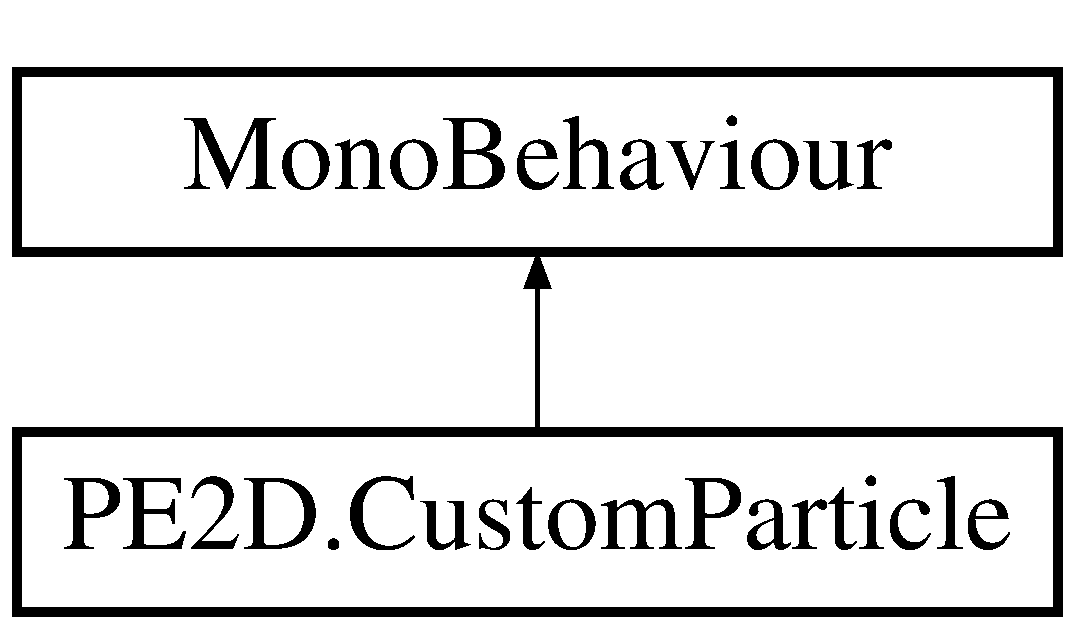
\includegraphics[height=2.000000cm]{class_p_e2_d_1_1_custom_particle}
\end{center}
\end{figure}
\subsection*{Static Public Member Functions}
\begin{DoxyCompactItemize}
\item 
static void \hyperlink{class_p_e2_d_1_1_custom_particle_aa49ae6d77d9160f453efa3826da35564}{Update\+Effector\+List} ()
\begin{DoxyCompactList}\small\item\em Finds all effectors in scene. Static reference should only be called once for all particles on effector change. \end{DoxyCompactList}\end{DoxyCompactItemize}
\subsection*{Public Attributes}
\begin{DoxyCompactItemize}
\item 
bool \hyperlink{class_p_e2_d_1_1_custom_particle_ad82465196a455ef29ff5c8e8c528c9b8}{should\+Update\+Alpha} = true
\begin{DoxyCompactList}\small\item\em Update sprites alpha based on velovity. \end{DoxyCompactList}\item 
bool \hyperlink{class_p_e2_d_1_1_custom_particle_a13a2f64584e65a38d7ec7b27f1d3fcd2}{should\+Update\+Scale} = true
\begin{DoxyCompactList}\small\item\em Update sprites scale based on velicoty. \end{DoxyCompactList}\end{DoxyCompactItemize}
\subsection*{Properties}
\begin{DoxyCompactItemize}
\item 
\hyperlink{struct_p_e2_d_1_1_particle_builder}{Particle\+Builder} \hyperlink{class_p_e2_d_1_1_custom_particle_a70eb3430c0338b4c69e7f90206814e08}{state}\hspace{0.3cm}{\ttfamily  \mbox{[}set\mbox{]}}
\begin{DoxyCompactList}\small\item\em Set the state of the particles. Also resets particles properties. \end{DoxyCompactList}\item 
float \hyperlink{class_p_e2_d_1_1_custom_particle_abb3aec5eef9b58cf98c6000da1ad732e}{duration}\hspace{0.3cm}{\ttfamily  \mbox{[}get, set\mbox{]}}
\begin{DoxyCompactList}\small\item\em Maximum duration of particles life. Life may be shorter dependent on velocity. \end{DoxyCompactList}\item 
float \hyperlink{class_p_e2_d_1_1_custom_particle_ab8a4cc9c8de193c92fecb50634358823}{percent\+Life}\hspace{0.3cm}{\ttfamily  \mbox{[}get, set\mbox{]}}
\begin{DoxyCompactList}\small\item\em Range (0, 1). 0 = time to remove from scene, 1 = just spawned. \end{DoxyCompactList}\item 
Sprite\+Renderer \hyperlink{class_p_e2_d_1_1_custom_particle_a6a116a174bdc1007d31528712f19aa7f}{sprite\+Renderer}\hspace{0.3cm}{\ttfamily  \mbox{[}get\mbox{]}}
\begin{DoxyCompactList}\small\item\em Gets the sprite renderer. \end{DoxyCompactList}\end{DoxyCompactItemize}


\subsection{Detailed Description}
Main workhorse for the custom particles. Updates particles state (colour, position, velocity etc), handles interaction with effectors, and applys any screen constraints. 



\subsection{Member Function Documentation}
\hypertarget{class_p_e2_d_1_1_custom_particle_aa49ae6d77d9160f453efa3826da35564}{}\index{P\+E2\+D\+::\+Custom\+Particle@{P\+E2\+D\+::\+Custom\+Particle}!Update\+Effector\+List@{Update\+Effector\+List}}
\index{Update\+Effector\+List@{Update\+Effector\+List}!P\+E2\+D\+::\+Custom\+Particle@{P\+E2\+D\+::\+Custom\+Particle}}
\subsubsection[{Update\+Effector\+List()}]{\setlength{\rightskip}{0pt plus 5cm}static void P\+E2\+D.\+Custom\+Particle.\+Update\+Effector\+List (
\begin{DoxyParamCaption}
{}
\end{DoxyParamCaption}
)\hspace{0.3cm}{\ttfamily [static]}}\label{class_p_e2_d_1_1_custom_particle_aa49ae6d77d9160f453efa3826da35564}


Finds all effectors in scene. Static reference should only be called once for all particles on effector change. 



\subsection{Member Data Documentation}
\hypertarget{class_p_e2_d_1_1_custom_particle_ad82465196a455ef29ff5c8e8c528c9b8}{}\index{P\+E2\+D\+::\+Custom\+Particle@{P\+E2\+D\+::\+Custom\+Particle}!should\+Update\+Alpha@{should\+Update\+Alpha}}
\index{should\+Update\+Alpha@{should\+Update\+Alpha}!P\+E2\+D\+::\+Custom\+Particle@{P\+E2\+D\+::\+Custom\+Particle}}
\subsubsection[{should\+Update\+Alpha}]{\setlength{\rightskip}{0pt plus 5cm}bool P\+E2\+D.\+Custom\+Particle.\+should\+Update\+Alpha = true}\label{class_p_e2_d_1_1_custom_particle_ad82465196a455ef29ff5c8e8c528c9b8}


Update sprites alpha based on velovity. 

\hypertarget{class_p_e2_d_1_1_custom_particle_a13a2f64584e65a38d7ec7b27f1d3fcd2}{}\index{P\+E2\+D\+::\+Custom\+Particle@{P\+E2\+D\+::\+Custom\+Particle}!should\+Update\+Scale@{should\+Update\+Scale}}
\index{should\+Update\+Scale@{should\+Update\+Scale}!P\+E2\+D\+::\+Custom\+Particle@{P\+E2\+D\+::\+Custom\+Particle}}
\subsubsection[{should\+Update\+Scale}]{\setlength{\rightskip}{0pt plus 5cm}bool P\+E2\+D.\+Custom\+Particle.\+should\+Update\+Scale = true}\label{class_p_e2_d_1_1_custom_particle_a13a2f64584e65a38d7ec7b27f1d3fcd2}


Update sprites scale based on velicoty. 



\subsection{Property Documentation}
\hypertarget{class_p_e2_d_1_1_custom_particle_abb3aec5eef9b58cf98c6000da1ad732e}{}\index{P\+E2\+D\+::\+Custom\+Particle@{P\+E2\+D\+::\+Custom\+Particle}!duration@{duration}}
\index{duration@{duration}!P\+E2\+D\+::\+Custom\+Particle@{P\+E2\+D\+::\+Custom\+Particle}}
\subsubsection[{duration}]{\setlength{\rightskip}{0pt plus 5cm}float P\+E2\+D.\+Custom\+Particle.\+duration\hspace{0.3cm}{\ttfamily [get]}, {\ttfamily [set]}}\label{class_p_e2_d_1_1_custom_particle_abb3aec5eef9b58cf98c6000da1ad732e}


Maximum duration of particles life. Life may be shorter dependent on velocity. 

The duration.\hypertarget{class_p_e2_d_1_1_custom_particle_ab8a4cc9c8de193c92fecb50634358823}{}\index{P\+E2\+D\+::\+Custom\+Particle@{P\+E2\+D\+::\+Custom\+Particle}!percent\+Life@{percent\+Life}}
\index{percent\+Life@{percent\+Life}!P\+E2\+D\+::\+Custom\+Particle@{P\+E2\+D\+::\+Custom\+Particle}}
\subsubsection[{percent\+Life}]{\setlength{\rightskip}{0pt plus 5cm}float P\+E2\+D.\+Custom\+Particle.\+percent\+Life\hspace{0.3cm}{\ttfamily [get]}, {\ttfamily [set]}}\label{class_p_e2_d_1_1_custom_particle_ab8a4cc9c8de193c92fecb50634358823}


Range (0, 1). 0 = time to remove from scene, 1 = just spawned. 

The percent life.\hypertarget{class_p_e2_d_1_1_custom_particle_a6a116a174bdc1007d31528712f19aa7f}{}\index{P\+E2\+D\+::\+Custom\+Particle@{P\+E2\+D\+::\+Custom\+Particle}!sprite\+Renderer@{sprite\+Renderer}}
\index{sprite\+Renderer@{sprite\+Renderer}!P\+E2\+D\+::\+Custom\+Particle@{P\+E2\+D\+::\+Custom\+Particle}}
\subsubsection[{sprite\+Renderer}]{\setlength{\rightskip}{0pt plus 5cm}Sprite\+Renderer P\+E2\+D.\+Custom\+Particle.\+sprite\+Renderer\hspace{0.3cm}{\ttfamily [get]}}\label{class_p_e2_d_1_1_custom_particle_a6a116a174bdc1007d31528712f19aa7f}


Gets the sprite renderer. 

The sprite renderer.\hypertarget{class_p_e2_d_1_1_custom_particle_a70eb3430c0338b4c69e7f90206814e08}{}\index{P\+E2\+D\+::\+Custom\+Particle@{P\+E2\+D\+::\+Custom\+Particle}!state@{state}}
\index{state@{state}!P\+E2\+D\+::\+Custom\+Particle@{P\+E2\+D\+::\+Custom\+Particle}}
\subsubsection[{state}]{\setlength{\rightskip}{0pt plus 5cm}{\bf Particle\+Builder} P\+E2\+D.\+Custom\+Particle.\+state\hspace{0.3cm}{\ttfamily [set]}}\label{class_p_e2_d_1_1_custom_particle_a70eb3430c0338b4c69e7f90206814e08}


Set the state of the particles. Also resets particles properties. 

The state.

The documentation for this class was generated from the following file\+:\begin{DoxyCompactItemize}
\item 
/\+Users/robert/\+Dropbox/\+Work/\+Unity/\+Particle Effects 2\+D/\+Assets/\+P\+E2\+D/\+Scripts/\+Particles/Custom\+Particle.\+cs\end{DoxyCompactItemize}

\hypertarget{class_p_e2_d_1_1_custom_particle_emitter}{}\section{P\+E2\+D.\+Custom\+Particle\+Emitter Class Reference}
\label{class_p_e2_d_1_1_custom_particle_emitter}\index{P\+E2\+D.\+Custom\+Particle\+Emitter@{P\+E2\+D.\+Custom\+Particle\+Emitter}}


Base class for \hyperlink{class_p_e2_d_1_1_particle_emitter_in_random_direction}{Particle\+Emitter\+In\+Random\+Direction} and \hyperlink{class_p_e2_d_1_1_particle_emitter_in_object_direction}{Particle\+Emitter\+In\+Object\+Direction}. Add base classes to Game\+Objects to easily create particle emitters.  


Inheritance diagram for P\+E2\+D.\+Custom\+Particle\+Emitter\+:\begin{figure}[H]
\begin{center}
\leavevmode
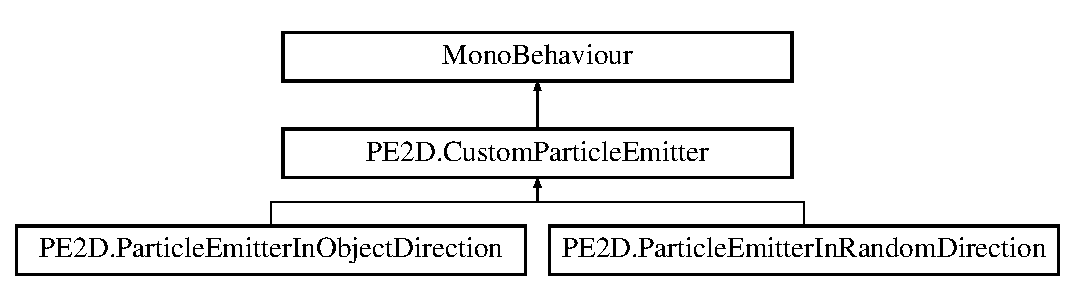
\includegraphics[height=3.000000cm]{class_p_e2_d_1_1_custom_particle_emitter}
\end{center}
\end{figure}
\subsection*{Public Member Functions}
\begin{DoxyCompactItemize}
\item 
void \hyperlink{class_p_e2_d_1_1_custom_particle_emitter_ab3e25c169bd7782b2982daab30e35bb8}{Turn\+On} ()
\begin{DoxyCompactList}\small\item\em Enables particle emission from this object. \end{DoxyCompactList}\item 
void \hyperlink{class_p_e2_d_1_1_custom_particle_emitter_a95849554a11e3072101bc3a74ea249af}{Turn\+Off} ()
\begin{DoxyCompactList}\small\item\em Disables particle emission from this object. \end{DoxyCompactList}\end{DoxyCompactItemize}
\subsection*{Public Attributes}
\begin{DoxyCompactItemize}
\item 
float \hyperlink{class_p_e2_d_1_1_custom_particle_emitter_a87bb71bb6472767b7532a19daa0d37e6}{time\+Between\+Projectile\+Release} = 0f
\begin{DoxyCompactList}\small\item\em The time between projectile release, if equals 0 then particle is released with each call to update. \end{DoxyCompactList}\item 
Vector2 \hyperlink{class_p_e2_d_1_1_custom_particle_emitter_a30b68ba2956245b5e75b81aee52ef0f1}{initial\+Scale} = new Vector2 (2f, 1f)
\begin{DoxyCompactList}\small\item\em Initial scale of the particles released. Scale is also dependent on velocity. \end{DoxyCompactList}\item 
bool \hyperlink{class_p_e2_d_1_1_custom_particle_emitter_a502b91bc7626becb13d2d908f8cc679d}{particles\+Enabled} = true
\begin{DoxyCompactList}\small\item\em Turns on/off particle generation from this Game\+Object. \end{DoxyCompactList}\item 
float \hyperlink{class_p_e2_d_1_1_custom_particle_emitter_a9dea38f5fcd24b14763dd9d7fc26cb7a}{duration} = 90f
\begin{DoxyCompactList}\small\item\em The maximum duration for each particle. A particles life is also dependent on velocity. \end{DoxyCompactList}\item 
float \hyperlink{class_p_e2_d_1_1_custom_particle_emitter_a04f3d21e5ff2436efce1e0f1a8777b03}{velocity\+Dampener} = 0.\+94f
\begin{DoxyCompactList}\small\item\em T\+He rate at which to reduce particles velocity each time step. \end{DoxyCompactList}\item 
float \hyperlink{class_p_e2_d_1_1_custom_particle_emitter_aaf85215c89bfa7e36482394c042af95e}{length\+Multiplier} = 40f
\begin{DoxyCompactList}\small\item\em The length multiplier for the particles. \end{DoxyCompactList}\item 
\hyperlink{namespace_p_e2_d_a510b407ed8d0de3476df258ab95e1e50}{Wrap\+Around\+Type} \hyperlink{class_p_e2_d_1_1_custom_particle_emitter_a894bcd6445f3443f1261ae98b50d097d}{wrap\+Around} = Wrap\+Around\+Type.\+None
\begin{DoxyCompactList}\small\item\em The screen constraint type. \end{DoxyCompactList}\item 
bool \hyperlink{class_p_e2_d_1_1_custom_particle_emitter_a2434866e0ea2e419987a2321f2455b3c}{random\+Colour} = false
\begin{DoxyCompactList}\small\item\em Particle will spawn as a random colour when enabled. \end{DoxyCompactList}\item 
Color \hyperlink{class_p_e2_d_1_1_custom_particle_emitter_a1ceaf22fc2d96bb356dfc6c86b6d2d66}{particle\+Colour}
\begin{DoxyCompactList}\small\item\em Set the particles colour. \end{DoxyCompactList}\item 
bool \hyperlink{class_p_e2_d_1_1_custom_particle_emitter_ab860a5e7888aa0c849a9815e3934bc7f}{clamp\+Min\+Length}
\begin{DoxyCompactList}\small\item\em Clamp the minimum length of a particle. \end{DoxyCompactList}\item 
float \hyperlink{class_p_e2_d_1_1_custom_particle_emitter_aaea8df4050265a7c0e07a35b9c9fde0e}{min\+Length}
\begin{DoxyCompactList}\small\item\em The minimum length of a particle, only used if \hyperlink{class_p_e2_d_1_1_custom_particle_emitter_ab860a5e7888aa0c849a9815e3934bc7f}{clamp\+Min\+Length} = true. \end{DoxyCompactList}\item 
bool \hyperlink{class_p_e2_d_1_1_custom_particle_emitter_a68678a550300ff27596c7d667df2d4f2}{clamp\+Max\+Length}
\begin{DoxyCompactList}\small\item\em Clamp the maximum length of a particle. \end{DoxyCompactList}\item 
float \hyperlink{class_p_e2_d_1_1_custom_particle_emitter_a88aef32381d4e9931fe75769bde81beb}{max\+Length}
\begin{DoxyCompactList}\small\item\em The minimum length of a particle, only used if \hyperlink{class_p_e2_d_1_1_custom_particle_emitter_a68678a550300ff27596c7d667df2d4f2}{clamp\+Max\+Length} = true. \end{DoxyCompactList}\item 
bool \hyperlink{class_p_e2_d_1_1_custom_particle_emitter_ad533ffa87500059c24f4883b4258ef1c}{remove\+When\+Velocity\+Reaches\+Threshold}
\begin{DoxyCompactList}\small\item\em Will remove a particle if velocity reaches a threshold. \end{DoxyCompactList}\item 
float \hyperlink{class_p_e2_d_1_1_custom_particle_emitter_adb6bfa354cb3cad1123ea63b6d8696b5}{custom\+Velocity\+Threshold}
\begin{DoxyCompactList}\small\item\em The velocity at which a particle will be removed, only used if \hyperlink{class_p_e2_d_1_1_custom_particle_emitter_ad533ffa87500059c24f4883b4258ef1c}{remove\+When\+Velocity\+Reaches\+Threshold} = true. \end{DoxyCompactList}\item 
bool \hyperlink{class_p_e2_d_1_1_custom_particle_emitter_a2d9f43eacfbc11f6fcfb546985ca9291}{remove\+When\+Alpha\+Reaches\+Threshold}
\begin{DoxyCompactList}\small\item\em Will remove the particle when its alpha reaches a specified threshold. \end{DoxyCompactList}\item 
float \hyperlink{class_p_e2_d_1_1_custom_particle_emitter_a7bbf2eca6359446ab220db98001ca1aa}{custom\+Alpha\+Threshold}
\begin{DoxyCompactList}\small\item\em The particles sprites alpha threshold at which a particle will be removed, only used if \hyperlink{class_p_e2_d_1_1_custom_particle_emitter_a2d9f43eacfbc11f6fcfb546985ca9291}{remove\+When\+Alpha\+Reaches\+Threshold} = true. \end{DoxyCompactList}\end{DoxyCompactItemize}
\subsection*{Protected Member Functions}
\begin{DoxyCompactItemize}
\item 
\hypertarget{class_p_e2_d_1_1_custom_particle_emitter_a8acdd831f0a9826372f1364dc95bbd68}{}Color {\bfseries Get\+Random\+Colour} ()\label{class_p_e2_d_1_1_custom_particle_emitter_a8acdd831f0a9826372f1364dc95bbd68}

\item 
\hypertarget{class_p_e2_d_1_1_custom_particle_emitter_a523ecc6d970a14bf1dfe76aa1cf55060}{}abstract void {\bfseries Release\+Particle} ()\label{class_p_e2_d_1_1_custom_particle_emitter_a523ecc6d970a14bf1dfe76aa1cf55060}

\end{DoxyCompactItemize}
\subsection*{Protected Attributes}
\begin{DoxyCompactItemize}
\item 
\hypertarget{class_p_e2_d_1_1_custom_particle_emitter_a633106f8aa88c5d0cf798f45cd30d395}{}\hyperlink{struct_p_e2_d_1_1_particle_builder}{Particle\+Builder} {\bfseries \+\_\+cached\+State}\label{class_p_e2_d_1_1_custom_particle_emitter_a633106f8aa88c5d0cf798f45cd30d395}

\end{DoxyCompactItemize}


\subsection{Detailed Description}
Base class for \hyperlink{class_p_e2_d_1_1_particle_emitter_in_random_direction}{Particle\+Emitter\+In\+Random\+Direction} and \hyperlink{class_p_e2_d_1_1_particle_emitter_in_object_direction}{Particle\+Emitter\+In\+Object\+Direction}. Add base classes to Game\+Objects to easily create particle emitters. 



\subsection{Member Function Documentation}
\hypertarget{class_p_e2_d_1_1_custom_particle_emitter_a95849554a11e3072101bc3a74ea249af}{}\index{P\+E2\+D\+::\+Custom\+Particle\+Emitter@{P\+E2\+D\+::\+Custom\+Particle\+Emitter}!Turn\+Off@{Turn\+Off}}
\index{Turn\+Off@{Turn\+Off}!P\+E2\+D\+::\+Custom\+Particle\+Emitter@{P\+E2\+D\+::\+Custom\+Particle\+Emitter}}
\subsubsection[{Turn\+Off()}]{\setlength{\rightskip}{0pt plus 5cm}void P\+E2\+D.\+Custom\+Particle\+Emitter.\+Turn\+Off (
\begin{DoxyParamCaption}
{}
\end{DoxyParamCaption}
)}\label{class_p_e2_d_1_1_custom_particle_emitter_a95849554a11e3072101bc3a74ea249af}


Disables particle emission from this object. 

\hypertarget{class_p_e2_d_1_1_custom_particle_emitter_ab3e25c169bd7782b2982daab30e35bb8}{}\index{P\+E2\+D\+::\+Custom\+Particle\+Emitter@{P\+E2\+D\+::\+Custom\+Particle\+Emitter}!Turn\+On@{Turn\+On}}
\index{Turn\+On@{Turn\+On}!P\+E2\+D\+::\+Custom\+Particle\+Emitter@{P\+E2\+D\+::\+Custom\+Particle\+Emitter}}
\subsubsection[{Turn\+On()}]{\setlength{\rightskip}{0pt plus 5cm}void P\+E2\+D.\+Custom\+Particle\+Emitter.\+Turn\+On (
\begin{DoxyParamCaption}
{}
\end{DoxyParamCaption}
)}\label{class_p_e2_d_1_1_custom_particle_emitter_ab3e25c169bd7782b2982daab30e35bb8}


Enables particle emission from this object. 



\subsection{Member Data Documentation}
\hypertarget{class_p_e2_d_1_1_custom_particle_emitter_a68678a550300ff27596c7d667df2d4f2}{}\index{P\+E2\+D\+::\+Custom\+Particle\+Emitter@{P\+E2\+D\+::\+Custom\+Particle\+Emitter}!clamp\+Max\+Length@{clamp\+Max\+Length}}
\index{clamp\+Max\+Length@{clamp\+Max\+Length}!P\+E2\+D\+::\+Custom\+Particle\+Emitter@{P\+E2\+D\+::\+Custom\+Particle\+Emitter}}
\subsubsection[{clamp\+Max\+Length}]{\setlength{\rightskip}{0pt plus 5cm}bool P\+E2\+D.\+Custom\+Particle\+Emitter.\+clamp\+Max\+Length}\label{class_p_e2_d_1_1_custom_particle_emitter_a68678a550300ff27596c7d667df2d4f2}


Clamp the maximum length of a particle. 

\hypertarget{class_p_e2_d_1_1_custom_particle_emitter_ab860a5e7888aa0c849a9815e3934bc7f}{}\index{P\+E2\+D\+::\+Custom\+Particle\+Emitter@{P\+E2\+D\+::\+Custom\+Particle\+Emitter}!clamp\+Min\+Length@{clamp\+Min\+Length}}
\index{clamp\+Min\+Length@{clamp\+Min\+Length}!P\+E2\+D\+::\+Custom\+Particle\+Emitter@{P\+E2\+D\+::\+Custom\+Particle\+Emitter}}
\subsubsection[{clamp\+Min\+Length}]{\setlength{\rightskip}{0pt plus 5cm}bool P\+E2\+D.\+Custom\+Particle\+Emitter.\+clamp\+Min\+Length}\label{class_p_e2_d_1_1_custom_particle_emitter_ab860a5e7888aa0c849a9815e3934bc7f}


Clamp the minimum length of a particle. 

\hypertarget{class_p_e2_d_1_1_custom_particle_emitter_a7bbf2eca6359446ab220db98001ca1aa}{}\index{P\+E2\+D\+::\+Custom\+Particle\+Emitter@{P\+E2\+D\+::\+Custom\+Particle\+Emitter}!custom\+Alpha\+Threshold@{custom\+Alpha\+Threshold}}
\index{custom\+Alpha\+Threshold@{custom\+Alpha\+Threshold}!P\+E2\+D\+::\+Custom\+Particle\+Emitter@{P\+E2\+D\+::\+Custom\+Particle\+Emitter}}
\subsubsection[{custom\+Alpha\+Threshold}]{\setlength{\rightskip}{0pt plus 5cm}float P\+E2\+D.\+Custom\+Particle\+Emitter.\+custom\+Alpha\+Threshold}\label{class_p_e2_d_1_1_custom_particle_emitter_a7bbf2eca6359446ab220db98001ca1aa}


The particles sprites alpha threshold at which a particle will be removed, only used if \hyperlink{class_p_e2_d_1_1_custom_particle_emitter_a2d9f43eacfbc11f6fcfb546985ca9291}{remove\+When\+Alpha\+Reaches\+Threshold} = true. 

\hypertarget{class_p_e2_d_1_1_custom_particle_emitter_adb6bfa354cb3cad1123ea63b6d8696b5}{}\index{P\+E2\+D\+::\+Custom\+Particle\+Emitter@{P\+E2\+D\+::\+Custom\+Particle\+Emitter}!custom\+Velocity\+Threshold@{custom\+Velocity\+Threshold}}
\index{custom\+Velocity\+Threshold@{custom\+Velocity\+Threshold}!P\+E2\+D\+::\+Custom\+Particle\+Emitter@{P\+E2\+D\+::\+Custom\+Particle\+Emitter}}
\subsubsection[{custom\+Velocity\+Threshold}]{\setlength{\rightskip}{0pt plus 5cm}float P\+E2\+D.\+Custom\+Particle\+Emitter.\+custom\+Velocity\+Threshold}\label{class_p_e2_d_1_1_custom_particle_emitter_adb6bfa354cb3cad1123ea63b6d8696b5}


The velocity at which a particle will be removed, only used if \hyperlink{class_p_e2_d_1_1_custom_particle_emitter_ad533ffa87500059c24f4883b4258ef1c}{remove\+When\+Velocity\+Reaches\+Threshold} = true. 

\hypertarget{class_p_e2_d_1_1_custom_particle_emitter_a9dea38f5fcd24b14763dd9d7fc26cb7a}{}\index{P\+E2\+D\+::\+Custom\+Particle\+Emitter@{P\+E2\+D\+::\+Custom\+Particle\+Emitter}!duration@{duration}}
\index{duration@{duration}!P\+E2\+D\+::\+Custom\+Particle\+Emitter@{P\+E2\+D\+::\+Custom\+Particle\+Emitter}}
\subsubsection[{duration}]{\setlength{\rightskip}{0pt plus 5cm}float P\+E2\+D.\+Custom\+Particle\+Emitter.\+duration = 90f}\label{class_p_e2_d_1_1_custom_particle_emitter_a9dea38f5fcd24b14763dd9d7fc26cb7a}


The maximum duration for each particle. A particles life is also dependent on velocity. 

\hypertarget{class_p_e2_d_1_1_custom_particle_emitter_a30b68ba2956245b5e75b81aee52ef0f1}{}\index{P\+E2\+D\+::\+Custom\+Particle\+Emitter@{P\+E2\+D\+::\+Custom\+Particle\+Emitter}!initial\+Scale@{initial\+Scale}}
\index{initial\+Scale@{initial\+Scale}!P\+E2\+D\+::\+Custom\+Particle\+Emitter@{P\+E2\+D\+::\+Custom\+Particle\+Emitter}}
\subsubsection[{initial\+Scale}]{\setlength{\rightskip}{0pt plus 5cm}Vector2 P\+E2\+D.\+Custom\+Particle\+Emitter.\+initial\+Scale = new Vector2 (2f, 1f)}\label{class_p_e2_d_1_1_custom_particle_emitter_a30b68ba2956245b5e75b81aee52ef0f1}


Initial scale of the particles released. Scale is also dependent on velocity. 

\hypertarget{class_p_e2_d_1_1_custom_particle_emitter_aaf85215c89bfa7e36482394c042af95e}{}\index{P\+E2\+D\+::\+Custom\+Particle\+Emitter@{P\+E2\+D\+::\+Custom\+Particle\+Emitter}!length\+Multiplier@{length\+Multiplier}}
\index{length\+Multiplier@{length\+Multiplier}!P\+E2\+D\+::\+Custom\+Particle\+Emitter@{P\+E2\+D\+::\+Custom\+Particle\+Emitter}}
\subsubsection[{length\+Multiplier}]{\setlength{\rightskip}{0pt plus 5cm}float P\+E2\+D.\+Custom\+Particle\+Emitter.\+length\+Multiplier = 40f}\label{class_p_e2_d_1_1_custom_particle_emitter_aaf85215c89bfa7e36482394c042af95e}


The length multiplier for the particles. 

\hypertarget{class_p_e2_d_1_1_custom_particle_emitter_a88aef32381d4e9931fe75769bde81beb}{}\index{P\+E2\+D\+::\+Custom\+Particle\+Emitter@{P\+E2\+D\+::\+Custom\+Particle\+Emitter}!max\+Length@{max\+Length}}
\index{max\+Length@{max\+Length}!P\+E2\+D\+::\+Custom\+Particle\+Emitter@{P\+E2\+D\+::\+Custom\+Particle\+Emitter}}
\subsubsection[{max\+Length}]{\setlength{\rightskip}{0pt plus 5cm}float P\+E2\+D.\+Custom\+Particle\+Emitter.\+max\+Length}\label{class_p_e2_d_1_1_custom_particle_emitter_a88aef32381d4e9931fe75769bde81beb}


The minimum length of a particle, only used if \hyperlink{class_p_e2_d_1_1_custom_particle_emitter_a68678a550300ff27596c7d667df2d4f2}{clamp\+Max\+Length} = true. 

\hypertarget{class_p_e2_d_1_1_custom_particle_emitter_aaea8df4050265a7c0e07a35b9c9fde0e}{}\index{P\+E2\+D\+::\+Custom\+Particle\+Emitter@{P\+E2\+D\+::\+Custom\+Particle\+Emitter}!min\+Length@{min\+Length}}
\index{min\+Length@{min\+Length}!P\+E2\+D\+::\+Custom\+Particle\+Emitter@{P\+E2\+D\+::\+Custom\+Particle\+Emitter}}
\subsubsection[{min\+Length}]{\setlength{\rightskip}{0pt plus 5cm}float P\+E2\+D.\+Custom\+Particle\+Emitter.\+min\+Length}\label{class_p_e2_d_1_1_custom_particle_emitter_aaea8df4050265a7c0e07a35b9c9fde0e}


The minimum length of a particle, only used if \hyperlink{class_p_e2_d_1_1_custom_particle_emitter_ab860a5e7888aa0c849a9815e3934bc7f}{clamp\+Min\+Length} = true. 

\hypertarget{class_p_e2_d_1_1_custom_particle_emitter_a1ceaf22fc2d96bb356dfc6c86b6d2d66}{}\index{P\+E2\+D\+::\+Custom\+Particle\+Emitter@{P\+E2\+D\+::\+Custom\+Particle\+Emitter}!particle\+Colour@{particle\+Colour}}
\index{particle\+Colour@{particle\+Colour}!P\+E2\+D\+::\+Custom\+Particle\+Emitter@{P\+E2\+D\+::\+Custom\+Particle\+Emitter}}
\subsubsection[{particle\+Colour}]{\setlength{\rightskip}{0pt plus 5cm}Color P\+E2\+D.\+Custom\+Particle\+Emitter.\+particle\+Colour}\label{class_p_e2_d_1_1_custom_particle_emitter_a1ceaf22fc2d96bb356dfc6c86b6d2d66}


Set the particles colour. 

\hypertarget{class_p_e2_d_1_1_custom_particle_emitter_a502b91bc7626becb13d2d908f8cc679d}{}\index{P\+E2\+D\+::\+Custom\+Particle\+Emitter@{P\+E2\+D\+::\+Custom\+Particle\+Emitter}!particles\+Enabled@{particles\+Enabled}}
\index{particles\+Enabled@{particles\+Enabled}!P\+E2\+D\+::\+Custom\+Particle\+Emitter@{P\+E2\+D\+::\+Custom\+Particle\+Emitter}}
\subsubsection[{particles\+Enabled}]{\setlength{\rightskip}{0pt plus 5cm}bool P\+E2\+D.\+Custom\+Particle\+Emitter.\+particles\+Enabled = true}\label{class_p_e2_d_1_1_custom_particle_emitter_a502b91bc7626becb13d2d908f8cc679d}


Turns on/off particle generation from this Game\+Object. 

\hypertarget{class_p_e2_d_1_1_custom_particle_emitter_a2434866e0ea2e419987a2321f2455b3c}{}\index{P\+E2\+D\+::\+Custom\+Particle\+Emitter@{P\+E2\+D\+::\+Custom\+Particle\+Emitter}!random\+Colour@{random\+Colour}}
\index{random\+Colour@{random\+Colour}!P\+E2\+D\+::\+Custom\+Particle\+Emitter@{P\+E2\+D\+::\+Custom\+Particle\+Emitter}}
\subsubsection[{random\+Colour}]{\setlength{\rightskip}{0pt plus 5cm}bool P\+E2\+D.\+Custom\+Particle\+Emitter.\+random\+Colour = false}\label{class_p_e2_d_1_1_custom_particle_emitter_a2434866e0ea2e419987a2321f2455b3c}


Particle will spawn as a random colour when enabled. 

\hypertarget{class_p_e2_d_1_1_custom_particle_emitter_a2d9f43eacfbc11f6fcfb546985ca9291}{}\index{P\+E2\+D\+::\+Custom\+Particle\+Emitter@{P\+E2\+D\+::\+Custom\+Particle\+Emitter}!remove\+When\+Alpha\+Reaches\+Threshold@{remove\+When\+Alpha\+Reaches\+Threshold}}
\index{remove\+When\+Alpha\+Reaches\+Threshold@{remove\+When\+Alpha\+Reaches\+Threshold}!P\+E2\+D\+::\+Custom\+Particle\+Emitter@{P\+E2\+D\+::\+Custom\+Particle\+Emitter}}
\subsubsection[{remove\+When\+Alpha\+Reaches\+Threshold}]{\setlength{\rightskip}{0pt plus 5cm}bool P\+E2\+D.\+Custom\+Particle\+Emitter.\+remove\+When\+Alpha\+Reaches\+Threshold}\label{class_p_e2_d_1_1_custom_particle_emitter_a2d9f43eacfbc11f6fcfb546985ca9291}


Will remove the particle when its alpha reaches a specified threshold. 

\hypertarget{class_p_e2_d_1_1_custom_particle_emitter_ad533ffa87500059c24f4883b4258ef1c}{}\index{P\+E2\+D\+::\+Custom\+Particle\+Emitter@{P\+E2\+D\+::\+Custom\+Particle\+Emitter}!remove\+When\+Velocity\+Reaches\+Threshold@{remove\+When\+Velocity\+Reaches\+Threshold}}
\index{remove\+When\+Velocity\+Reaches\+Threshold@{remove\+When\+Velocity\+Reaches\+Threshold}!P\+E2\+D\+::\+Custom\+Particle\+Emitter@{P\+E2\+D\+::\+Custom\+Particle\+Emitter}}
\subsubsection[{remove\+When\+Velocity\+Reaches\+Threshold}]{\setlength{\rightskip}{0pt plus 5cm}bool P\+E2\+D.\+Custom\+Particle\+Emitter.\+remove\+When\+Velocity\+Reaches\+Threshold}\label{class_p_e2_d_1_1_custom_particle_emitter_ad533ffa87500059c24f4883b4258ef1c}


Will remove a particle if velocity reaches a threshold. 

\hypertarget{class_p_e2_d_1_1_custom_particle_emitter_a87bb71bb6472767b7532a19daa0d37e6}{}\index{P\+E2\+D\+::\+Custom\+Particle\+Emitter@{P\+E2\+D\+::\+Custom\+Particle\+Emitter}!time\+Between\+Projectile\+Release@{time\+Between\+Projectile\+Release}}
\index{time\+Between\+Projectile\+Release@{time\+Between\+Projectile\+Release}!P\+E2\+D\+::\+Custom\+Particle\+Emitter@{P\+E2\+D\+::\+Custom\+Particle\+Emitter}}
\subsubsection[{time\+Between\+Projectile\+Release}]{\setlength{\rightskip}{0pt plus 5cm}float P\+E2\+D.\+Custom\+Particle\+Emitter.\+time\+Between\+Projectile\+Release = 0f}\label{class_p_e2_d_1_1_custom_particle_emitter_a87bb71bb6472767b7532a19daa0d37e6}


The time between projectile release, if equals 0 then particle is released with each call to update. 

\hypertarget{class_p_e2_d_1_1_custom_particle_emitter_a04f3d21e5ff2436efce1e0f1a8777b03}{}\index{P\+E2\+D\+::\+Custom\+Particle\+Emitter@{P\+E2\+D\+::\+Custom\+Particle\+Emitter}!velocity\+Dampener@{velocity\+Dampener}}
\index{velocity\+Dampener@{velocity\+Dampener}!P\+E2\+D\+::\+Custom\+Particle\+Emitter@{P\+E2\+D\+::\+Custom\+Particle\+Emitter}}
\subsubsection[{velocity\+Dampener}]{\setlength{\rightskip}{0pt plus 5cm}float P\+E2\+D.\+Custom\+Particle\+Emitter.\+velocity\+Dampener = 0.\+94f}\label{class_p_e2_d_1_1_custom_particle_emitter_a04f3d21e5ff2436efce1e0f1a8777b03}


T\+He rate at which to reduce particles velocity each time step. 

\hypertarget{class_p_e2_d_1_1_custom_particle_emitter_a894bcd6445f3443f1261ae98b50d097d}{}\index{P\+E2\+D\+::\+Custom\+Particle\+Emitter@{P\+E2\+D\+::\+Custom\+Particle\+Emitter}!wrap\+Around@{wrap\+Around}}
\index{wrap\+Around@{wrap\+Around}!P\+E2\+D\+::\+Custom\+Particle\+Emitter@{P\+E2\+D\+::\+Custom\+Particle\+Emitter}}
\subsubsection[{wrap\+Around}]{\setlength{\rightskip}{0pt plus 5cm}{\bf Wrap\+Around\+Type} P\+E2\+D.\+Custom\+Particle\+Emitter.\+wrap\+Around = Wrap\+Around\+Type.\+None}\label{class_p_e2_d_1_1_custom_particle_emitter_a894bcd6445f3443f1261ae98b50d097d}


The screen constraint type. 



The documentation for this class was generated from the following file\+:\begin{DoxyCompactItemize}
\item 
/\+Users/robert/\+Dropbox/\+Work/\+Unity/\+Particle Effects 2\+D/\+Assets/\+P\+E2\+D/\+Scripts/\+Particles/\+Emitters/Custom\+Particle\+Emitter.\+cs\end{DoxyCompactItemize}

\hypertarget{class_demo_constraint_switcher}{}\section{Demo\+Constraint\+Switcher Class Reference}
\label{class_demo_constraint_switcher}\index{Demo\+Constraint\+Switcher@{Demo\+Constraint\+Switcher}}


Switches between screen constraints in the demo scene.  


Inheritance diagram for Demo\+Constraint\+Switcher\+:\begin{figure}[H]
\begin{center}
\leavevmode
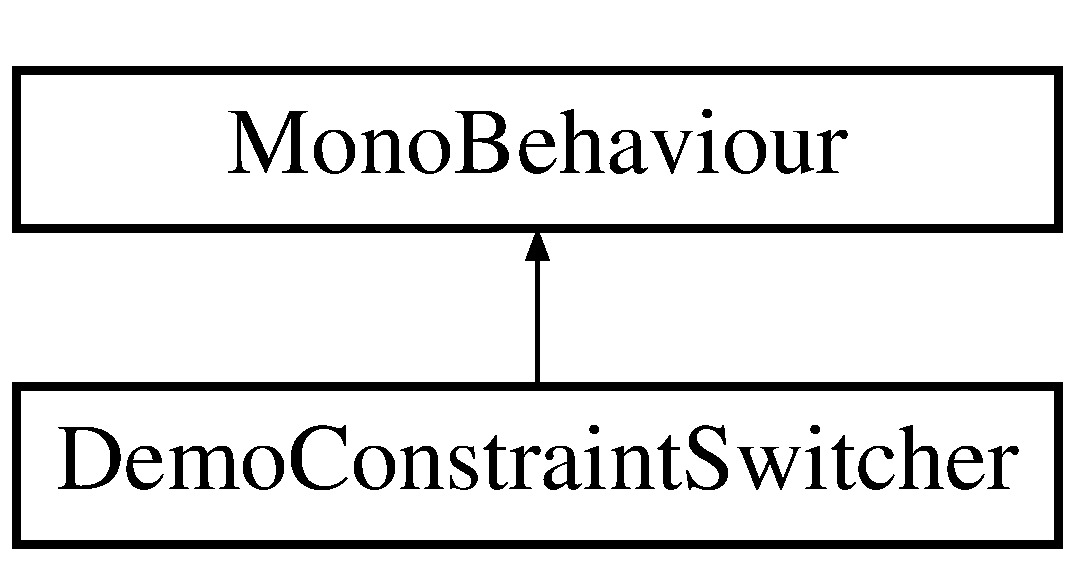
\includegraphics[height=2.000000cm]{class_demo_constraint_switcher}
\end{center}
\end{figure}
\subsection*{Public Attributes}
\begin{DoxyCompactItemize}
\item 
\hypertarget{class_demo_constraint_switcher_af43145389170ecb768eddb9385820529}{}\hyperlink{class_demo_mouse_controller}{Demo\+Mouse\+Controller} {\bfseries mouse\+Controller}\label{class_demo_constraint_switcher_af43145389170ecb768eddb9385820529}

\item 
\hypertarget{class_demo_constraint_switcher_ac5b5887291ba6e09aaac65000c48b067}{}Text {\bfseries constraint\+Text}\label{class_demo_constraint_switcher_ac5b5887291ba6e09aaac65000c48b067}

\end{DoxyCompactItemize}


\subsection{Detailed Description}
Switches between screen constraints in the demo scene. 



The documentation for this class was generated from the following file\+:\begin{DoxyCompactItemize}
\item 
/\+Users/robert/\+Dropbox/\+Work/\+Unity/\+Particle Effects 2\+D/\+Assets/\+P\+E2\+D/\+Scripts/\+Demo/Demo\+Constraint\+Switcher.\+cs\end{DoxyCompactItemize}

\hypertarget{class_demo_mouse_controller}{}\section{Demo\+Mouse\+Controller Class Reference}
\label{class_demo_mouse_controller}\index{Demo\+Mouse\+Controller@{Demo\+Mouse\+Controller}}


Spawns a circular explosion of particles on mouse click. Example of how to procedurally create particles.  


Inheritance diagram for Demo\+Mouse\+Controller\+:\begin{figure}[H]
\begin{center}
\leavevmode
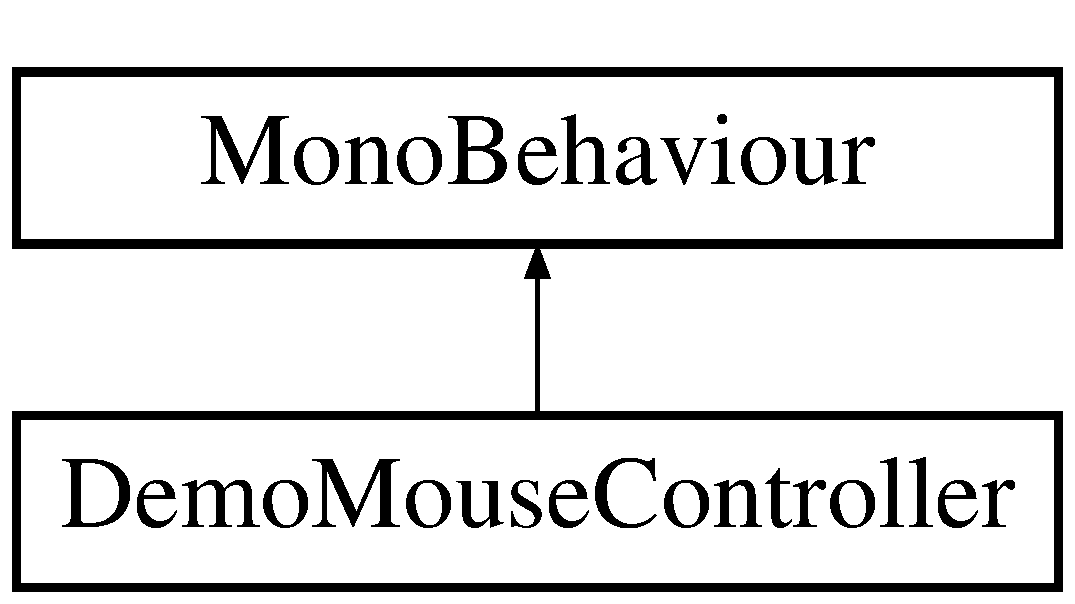
\includegraphics[height=2.000000cm]{class_demo_mouse_controller}
\end{center}
\end{figure}
\subsection*{Public Attributes}
\begin{DoxyCompactItemize}
\item 
\hypertarget{class_demo_mouse_controller_a1597c655ed4460c48dd430b89b36f3cc}{}float {\bfseries speed\+Offset} = .\+01f\label{class_demo_mouse_controller_a1597c655ed4460c48dd430b89b36f3cc}

\item 
\hypertarget{class_demo_mouse_controller_adf0cb01f16b5d543067a2013a057e288}{}float {\bfseries length\+Multiplier} = 40f\label{class_demo_mouse_controller_adf0cb01f16b5d543067a2013a057e288}

\item 
\hypertarget{class_demo_mouse_controller_aa1a4bf8c5555d83629b6c9bfe22fe578}{}int {\bfseries num\+To\+Spawn} = 200\label{class_demo_mouse_controller_aa1a4bf8c5555d83629b6c9bfe22fe578}

\item 
\hypertarget{class_demo_mouse_controller_ad1f203719d0f8be7eff222da2a8596ed}{}\hyperlink{namespace_p_e2_d_a510b407ed8d0de3476df258ab95e1e50}{Wrap\+Around\+Type} {\bfseries wrap\+Around}\label{class_demo_mouse_controller_ad1f203719d0f8be7eff222da2a8596ed}

\end{DoxyCompactItemize}


\subsection{Detailed Description}
Spawns a circular explosion of particles on mouse click. Example of how to procedurally create particles. 



The documentation for this class was generated from the following file\+:\begin{DoxyCompactItemize}
\item 
/\+Users/robert/\+Dropbox/\+Work/\+Unity/\+Particle Effects 2\+D/\+Assets/\+P\+E2\+D/\+Scripts/\+Demo/Demo\+Mouse\+Controller.\+cs\end{DoxyCompactItemize}

\hypertarget{class_demo_particle_emitter_switcher}{}\section{Demo\+Particle\+Emitter\+Switcher Class Reference}
\label{class_demo_particle_emitter_switcher}\index{Demo\+Particle\+Emitter\+Switcher@{Demo\+Particle\+Emitter\+Switcher}}


Switches between particle emitters in demo scene.  


Inheritance diagram for Demo\+Particle\+Emitter\+Switcher\+:\begin{figure}[H]
\begin{center}
\leavevmode
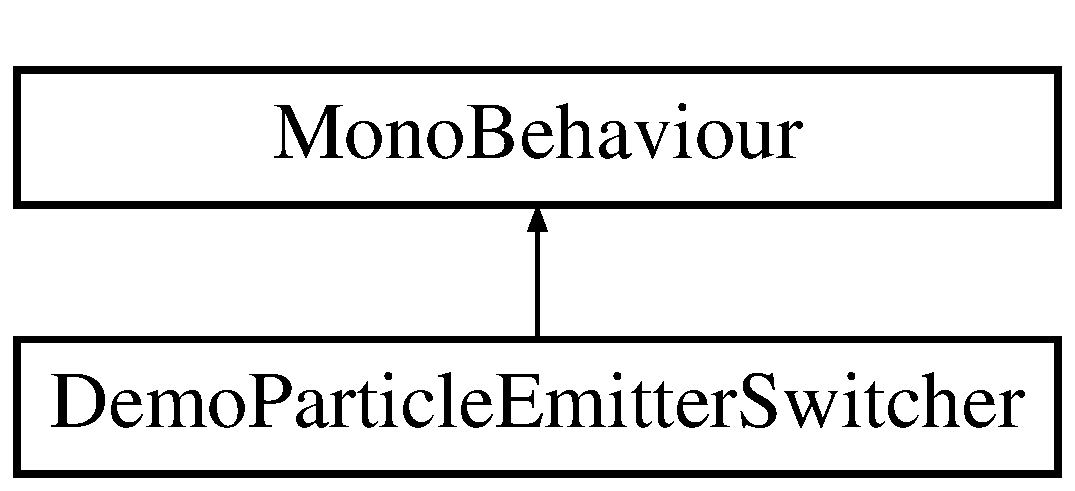
\includegraphics[height=2.000000cm]{class_demo_particle_emitter_switcher}
\end{center}
\end{figure}
\subsection*{Public Attributes}
\begin{DoxyCompactItemize}
\item 
\hypertarget{class_demo_particle_emitter_switcher_aaf0a3b5a20f6f79088d6d616aa09e0d7}{}Game\+Object\mbox{[}$\,$\mbox{]} {\bfseries particle\+Emitters}\label{class_demo_particle_emitter_switcher_aaf0a3b5a20f6f79088d6d616aa09e0d7}

\item 
\hypertarget{class_demo_particle_emitter_switcher_afb968986e985f571061aaf8b0838f0cd}{}Text {\bfseries emitter\+Text}\label{class_demo_particle_emitter_switcher_afb968986e985f571061aaf8b0838f0cd}

\item 
\hypertarget{class_demo_particle_emitter_switcher_a6f166dc96014592c56138d79dee4a740}{}string {\bfseries pre\+Emitter\+String}\label{class_demo_particle_emitter_switcher_a6f166dc96014592c56138d79dee4a740}

\item 
\hypertarget{class_demo_particle_emitter_switcher_ab8841c0c04141643617ed9dd3de8a3f6}{}string {\bfseries post\+Emitter\+String}\label{class_demo_particle_emitter_switcher_ab8841c0c04141643617ed9dd3de8a3f6}

\item 
\hypertarget{class_demo_particle_emitter_switcher_ac76a51e97ff6db549a765ef17c7cfac0}{}bool {\bfseries update\+Effectors\+On\+Change} = false\label{class_demo_particle_emitter_switcher_ac76a51e97ff6db549a765ef17c7cfac0}

\end{DoxyCompactItemize}


\subsection{Detailed Description}
Switches between particle emitters in demo scene. 



The documentation for this class was generated from the following file\+:\begin{DoxyCompactItemize}
\item 
/\+Users/robert/\+Dropbox/\+Work/\+Unity/\+Particle Effects 2\+D/\+Assets/\+P\+E2\+D/\+Scripts/\+Demo/Demo\+Particle\+Emitter\+Switcher.\+cs\end{DoxyCompactItemize}

\hypertarget{class_demo_scene_switcher}{}\section{Demo\+Scene\+Switcher Class Reference}
\label{class_demo_scene_switcher}\index{Demo\+Scene\+Switcher@{Demo\+Scene\+Switcher}}


Switches between demo scenes when enter key pressed.  


Inheritance diagram for Demo\+Scene\+Switcher\+:\begin{figure}[H]
\begin{center}
\leavevmode
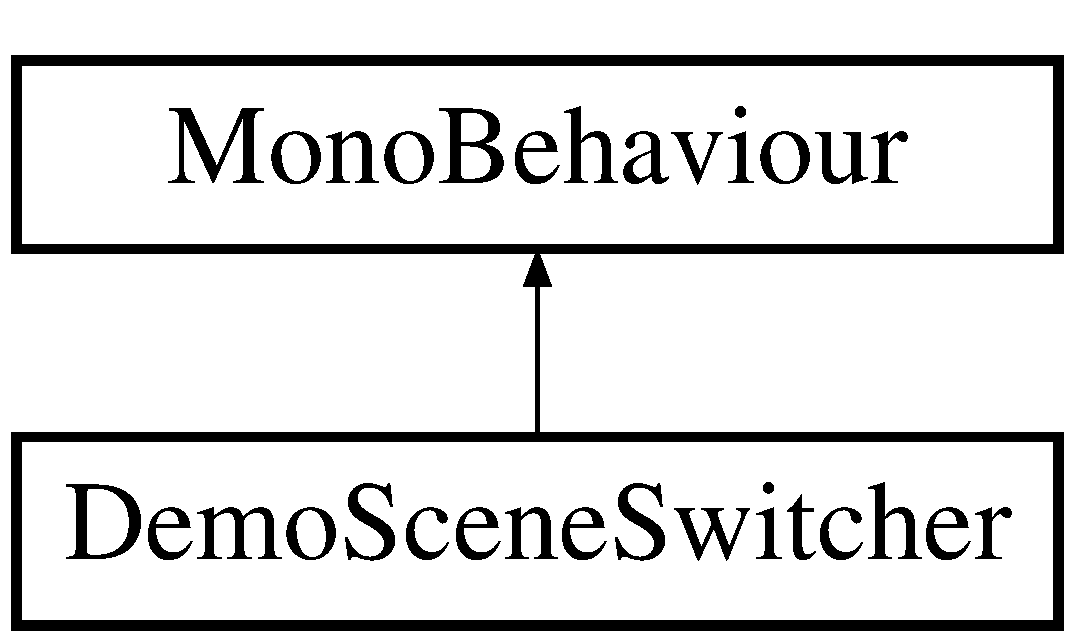
\includegraphics[height=2.000000cm]{class_demo_scene_switcher}
\end{center}
\end{figure}
\subsection*{Public Attributes}
\begin{DoxyCompactItemize}
\item 
\hypertarget{class_demo_scene_switcher_a761bbb8d1fbeb9f9f572f7677765dab8}{}int {\bfseries number\+Of\+Scenes} = 3\label{class_demo_scene_switcher_a761bbb8d1fbeb9f9f572f7677765dab8}

\end{DoxyCompactItemize}


\subsection{Detailed Description}
Switches between demo scenes when enter key pressed. 



The documentation for this class was generated from the following file\+:\begin{DoxyCompactItemize}
\item 
/\+Users/robert/\+Dropbox/\+Work/\+Unity/\+Particle Effects 2\+D/\+Assets/\+P\+E2\+D/\+Scripts/\+Demo/Demo\+Scene\+Switcher.\+cs\end{DoxyCompactItemize}

\hypertarget{struct_p_e2_d_1_1_particle_builder}{}\section{P\+E2\+D.\+Particle\+Builder Struct Reference}
\label{struct_p_e2_d_1_1_particle_builder}\index{P\+E2\+D.\+Particle\+Builder@{P\+E2\+D.\+Particle\+Builder}}


Holds the particle state. Passed to the \hyperlink{class_p_e2_d_1_1_particle_factory}{Particle\+Factory} to build particles.  


\subsection*{Public Attributes}
\begin{DoxyCompactItemize}
\item 
Vector2 \hyperlink{struct_p_e2_d_1_1_particle_builder_a5efd39fc998887c16fa23eff2fdf8d4d}{velocity}
\begin{DoxyCompactList}\small\item\em Initial velocity of particle. \end{DoxyCompactList}\item 
\hyperlink{namespace_p_e2_d_a510b407ed8d0de3476df258ab95e1e50}{Wrap\+Around\+Type} \hyperlink{struct_p_e2_d_1_1_particle_builder_ae8a54269a26406d7fb499c4fee198ea2}{wrap\+Around\+Type}
\begin{DoxyCompactList}\small\item\em Screen constraint type. \end{DoxyCompactList}\item 
float \hyperlink{struct_p_e2_d_1_1_particle_builder_a3079f1fec16ed4f3b83def7200345569}{length\+Multiplier}
\begin{DoxyCompactList}\small\item\em The particles scale is multipled by this. \end{DoxyCompactList}\item 
float \hyperlink{struct_p_e2_d_1_1_particle_builder_aff988495a250de55e362b008dc471f9d}{velocity\+Damp\+Modifier}
\begin{DoxyCompactList}\small\item\em The percentage amount that a particles velocity remains each timestep. \end{DoxyCompactList}\item 
bool \hyperlink{struct_p_e2_d_1_1_particle_builder_aa78452c0a3ec79744b768d945b1d6ae9}{ignore\+Effectors}
\begin{DoxyCompactList}\small\item\em If enables, the particle built with this state will ignore effectors. \end{DoxyCompactList}\item 
float \hyperlink{struct_p_e2_d_1_1_particle_builder_aff3a3bd2b886093998811a30e7a906fd}{min\+Length\+Clamp}
\begin{DoxyCompactList}\small\item\em Clamp the minimum length of a particles sprite. \end{DoxyCompactList}\item 
float \hyperlink{struct_p_e2_d_1_1_particle_builder_a80efc62ef75c9a7c127caa527e7c83ca}{max\+Length\+Clamp}
\begin{DoxyCompactList}\small\item\em Clamp the maximum length of a particles sprite. \end{DoxyCompactList}\item 
bool \hyperlink{struct_p_e2_d_1_1_particle_builder_a2c37b78b4c75113fb9703c760cd1a34c}{remove\+When\+Velocity\+Reaches\+Threshold}
\begin{DoxyCompactList}\small\item\em Will remove a particle if velocity reaches a threshold. \end{DoxyCompactList}\item 
float \hyperlink{struct_p_e2_d_1_1_particle_builder_a5feb3a73d241bbf14bd2a51ec94835b2}{custom\+Velocity\+Threshold}
\begin{DoxyCompactList}\small\item\em The velocity at which a particle will be removed, only used if \hyperlink{struct_p_e2_d_1_1_particle_builder_a2c37b78b4c75113fb9703c760cd1a34c}{remove\+When\+Velocity\+Reaches\+Threshold} = true. \end{DoxyCompactList}\item 
bool \hyperlink{struct_p_e2_d_1_1_particle_builder_a18a773bd0ec19ac1eeb2e86603bd3395}{remove\+When\+Alpha\+Reaches\+Threshold}
\begin{DoxyCompactList}\small\item\em Will remove the particle when its alpha reaches a specified threshold. \end{DoxyCompactList}\item 
float \hyperlink{struct_p_e2_d_1_1_particle_builder_a4f81feb8debd8a2842d2d1b49fa842e2}{custom\+Alpha\+Threshold}
\begin{DoxyCompactList}\small\item\em The particles sprites alpha threshold at which a particle will be removed, only used if \hyperlink{struct_p_e2_d_1_1_particle_builder_a18a773bd0ec19ac1eeb2e86603bd3395}{remove\+When\+Alpha\+Reaches\+Threshold} = true. \end{DoxyCompactList}\end{DoxyCompactItemize}


\subsection{Detailed Description}
Holds the particle state. Passed to the \hyperlink{class_p_e2_d_1_1_particle_factory}{Particle\+Factory} to build particles. 



\subsection{Member Data Documentation}
\hypertarget{struct_p_e2_d_1_1_particle_builder_a4f81feb8debd8a2842d2d1b49fa842e2}{}\index{P\+E2\+D\+::\+Particle\+Builder@{P\+E2\+D\+::\+Particle\+Builder}!custom\+Alpha\+Threshold@{custom\+Alpha\+Threshold}}
\index{custom\+Alpha\+Threshold@{custom\+Alpha\+Threshold}!P\+E2\+D\+::\+Particle\+Builder@{P\+E2\+D\+::\+Particle\+Builder}}
\subsubsection[{custom\+Alpha\+Threshold}]{\setlength{\rightskip}{0pt plus 5cm}float P\+E2\+D.\+Particle\+Builder.\+custom\+Alpha\+Threshold}\label{struct_p_e2_d_1_1_particle_builder_a4f81feb8debd8a2842d2d1b49fa842e2}


The particles sprites alpha threshold at which a particle will be removed, only used if \hyperlink{struct_p_e2_d_1_1_particle_builder_a18a773bd0ec19ac1eeb2e86603bd3395}{remove\+When\+Alpha\+Reaches\+Threshold} = true. 

\hypertarget{struct_p_e2_d_1_1_particle_builder_a5feb3a73d241bbf14bd2a51ec94835b2}{}\index{P\+E2\+D\+::\+Particle\+Builder@{P\+E2\+D\+::\+Particle\+Builder}!custom\+Velocity\+Threshold@{custom\+Velocity\+Threshold}}
\index{custom\+Velocity\+Threshold@{custom\+Velocity\+Threshold}!P\+E2\+D\+::\+Particle\+Builder@{P\+E2\+D\+::\+Particle\+Builder}}
\subsubsection[{custom\+Velocity\+Threshold}]{\setlength{\rightskip}{0pt plus 5cm}float P\+E2\+D.\+Particle\+Builder.\+custom\+Velocity\+Threshold}\label{struct_p_e2_d_1_1_particle_builder_a5feb3a73d241bbf14bd2a51ec94835b2}


The velocity at which a particle will be removed, only used if \hyperlink{struct_p_e2_d_1_1_particle_builder_a2c37b78b4c75113fb9703c760cd1a34c}{remove\+When\+Velocity\+Reaches\+Threshold} = true. 

\hypertarget{struct_p_e2_d_1_1_particle_builder_aa78452c0a3ec79744b768d945b1d6ae9}{}\index{P\+E2\+D\+::\+Particle\+Builder@{P\+E2\+D\+::\+Particle\+Builder}!ignore\+Effectors@{ignore\+Effectors}}
\index{ignore\+Effectors@{ignore\+Effectors}!P\+E2\+D\+::\+Particle\+Builder@{P\+E2\+D\+::\+Particle\+Builder}}
\subsubsection[{ignore\+Effectors}]{\setlength{\rightskip}{0pt plus 5cm}bool P\+E2\+D.\+Particle\+Builder.\+ignore\+Effectors}\label{struct_p_e2_d_1_1_particle_builder_aa78452c0a3ec79744b768d945b1d6ae9}


If enables, the particle built with this state will ignore effectors. 

\hypertarget{struct_p_e2_d_1_1_particle_builder_a3079f1fec16ed4f3b83def7200345569}{}\index{P\+E2\+D\+::\+Particle\+Builder@{P\+E2\+D\+::\+Particle\+Builder}!length\+Multiplier@{length\+Multiplier}}
\index{length\+Multiplier@{length\+Multiplier}!P\+E2\+D\+::\+Particle\+Builder@{P\+E2\+D\+::\+Particle\+Builder}}
\subsubsection[{length\+Multiplier}]{\setlength{\rightskip}{0pt plus 5cm}float P\+E2\+D.\+Particle\+Builder.\+length\+Multiplier}\label{struct_p_e2_d_1_1_particle_builder_a3079f1fec16ed4f3b83def7200345569}


The particles scale is multipled by this. 

\hypertarget{struct_p_e2_d_1_1_particle_builder_a80efc62ef75c9a7c127caa527e7c83ca}{}\index{P\+E2\+D\+::\+Particle\+Builder@{P\+E2\+D\+::\+Particle\+Builder}!max\+Length\+Clamp@{max\+Length\+Clamp}}
\index{max\+Length\+Clamp@{max\+Length\+Clamp}!P\+E2\+D\+::\+Particle\+Builder@{P\+E2\+D\+::\+Particle\+Builder}}
\subsubsection[{max\+Length\+Clamp}]{\setlength{\rightskip}{0pt plus 5cm}float P\+E2\+D.\+Particle\+Builder.\+max\+Length\+Clamp}\label{struct_p_e2_d_1_1_particle_builder_a80efc62ef75c9a7c127caa527e7c83ca}


Clamp the maximum length of a particles sprite. 

\hypertarget{struct_p_e2_d_1_1_particle_builder_aff3a3bd2b886093998811a30e7a906fd}{}\index{P\+E2\+D\+::\+Particle\+Builder@{P\+E2\+D\+::\+Particle\+Builder}!min\+Length\+Clamp@{min\+Length\+Clamp}}
\index{min\+Length\+Clamp@{min\+Length\+Clamp}!P\+E2\+D\+::\+Particle\+Builder@{P\+E2\+D\+::\+Particle\+Builder}}
\subsubsection[{min\+Length\+Clamp}]{\setlength{\rightskip}{0pt plus 5cm}float P\+E2\+D.\+Particle\+Builder.\+min\+Length\+Clamp}\label{struct_p_e2_d_1_1_particle_builder_aff3a3bd2b886093998811a30e7a906fd}


Clamp the minimum length of a particles sprite. 

\hypertarget{struct_p_e2_d_1_1_particle_builder_a18a773bd0ec19ac1eeb2e86603bd3395}{}\index{P\+E2\+D\+::\+Particle\+Builder@{P\+E2\+D\+::\+Particle\+Builder}!remove\+When\+Alpha\+Reaches\+Threshold@{remove\+When\+Alpha\+Reaches\+Threshold}}
\index{remove\+When\+Alpha\+Reaches\+Threshold@{remove\+When\+Alpha\+Reaches\+Threshold}!P\+E2\+D\+::\+Particle\+Builder@{P\+E2\+D\+::\+Particle\+Builder}}
\subsubsection[{remove\+When\+Alpha\+Reaches\+Threshold}]{\setlength{\rightskip}{0pt plus 5cm}bool P\+E2\+D.\+Particle\+Builder.\+remove\+When\+Alpha\+Reaches\+Threshold}\label{struct_p_e2_d_1_1_particle_builder_a18a773bd0ec19ac1eeb2e86603bd3395}


Will remove the particle when its alpha reaches a specified threshold. 

\hypertarget{struct_p_e2_d_1_1_particle_builder_a2c37b78b4c75113fb9703c760cd1a34c}{}\index{P\+E2\+D\+::\+Particle\+Builder@{P\+E2\+D\+::\+Particle\+Builder}!remove\+When\+Velocity\+Reaches\+Threshold@{remove\+When\+Velocity\+Reaches\+Threshold}}
\index{remove\+When\+Velocity\+Reaches\+Threshold@{remove\+When\+Velocity\+Reaches\+Threshold}!P\+E2\+D\+::\+Particle\+Builder@{P\+E2\+D\+::\+Particle\+Builder}}
\subsubsection[{remove\+When\+Velocity\+Reaches\+Threshold}]{\setlength{\rightskip}{0pt plus 5cm}bool P\+E2\+D.\+Particle\+Builder.\+remove\+When\+Velocity\+Reaches\+Threshold}\label{struct_p_e2_d_1_1_particle_builder_a2c37b78b4c75113fb9703c760cd1a34c}


Will remove a particle if velocity reaches a threshold. 

\hypertarget{struct_p_e2_d_1_1_particle_builder_a5efd39fc998887c16fa23eff2fdf8d4d}{}\index{P\+E2\+D\+::\+Particle\+Builder@{P\+E2\+D\+::\+Particle\+Builder}!velocity@{velocity}}
\index{velocity@{velocity}!P\+E2\+D\+::\+Particle\+Builder@{P\+E2\+D\+::\+Particle\+Builder}}
\subsubsection[{velocity}]{\setlength{\rightskip}{0pt plus 5cm}Vector2 P\+E2\+D.\+Particle\+Builder.\+velocity}\label{struct_p_e2_d_1_1_particle_builder_a5efd39fc998887c16fa23eff2fdf8d4d}


Initial velocity of particle. 

\hypertarget{struct_p_e2_d_1_1_particle_builder_aff988495a250de55e362b008dc471f9d}{}\index{P\+E2\+D\+::\+Particle\+Builder@{P\+E2\+D\+::\+Particle\+Builder}!velocity\+Damp\+Modifier@{velocity\+Damp\+Modifier}}
\index{velocity\+Damp\+Modifier@{velocity\+Damp\+Modifier}!P\+E2\+D\+::\+Particle\+Builder@{P\+E2\+D\+::\+Particle\+Builder}}
\subsubsection[{velocity\+Damp\+Modifier}]{\setlength{\rightskip}{0pt plus 5cm}float P\+E2\+D.\+Particle\+Builder.\+velocity\+Damp\+Modifier}\label{struct_p_e2_d_1_1_particle_builder_aff988495a250de55e362b008dc471f9d}


The percentage amount that a particles velocity remains each timestep. 

\hypertarget{struct_p_e2_d_1_1_particle_builder_ae8a54269a26406d7fb499c4fee198ea2}{}\index{P\+E2\+D\+::\+Particle\+Builder@{P\+E2\+D\+::\+Particle\+Builder}!wrap\+Around\+Type@{wrap\+Around\+Type}}
\index{wrap\+Around\+Type@{wrap\+Around\+Type}!P\+E2\+D\+::\+Particle\+Builder@{P\+E2\+D\+::\+Particle\+Builder}}
\subsubsection[{wrap\+Around\+Type}]{\setlength{\rightskip}{0pt plus 5cm}{\bf Wrap\+Around\+Type} P\+E2\+D.\+Particle\+Builder.\+wrap\+Around\+Type}\label{struct_p_e2_d_1_1_particle_builder_ae8a54269a26406d7fb499c4fee198ea2}


Screen constraint type. 



The documentation for this struct was generated from the following file\+:\begin{DoxyCompactItemize}
\item 
/\+Users/robert/\+Dropbox/\+Work/\+Unity/\+Particle Effects 2\+D/\+Assets/\+P\+E2\+D/\+Scripts/\+Particles/Particle\+Builder.\+cs\end{DoxyCompactItemize}

\hypertarget{class_p_e2_d_1_1_particle_effector}{}\section{P\+E2\+D.\+Particle\+Effector Class Reference}
\label{class_p_e2_d_1_1_particle_effector}\index{P\+E2\+D.\+Particle\+Effector@{P\+E2\+D.\+Particle\+Effector}}


Add to a gameobject to effect a particles movement.  


Inheritance diagram for P\+E2\+D.\+Particle\+Effector\+:\begin{figure}[H]
\begin{center}
\leavevmode
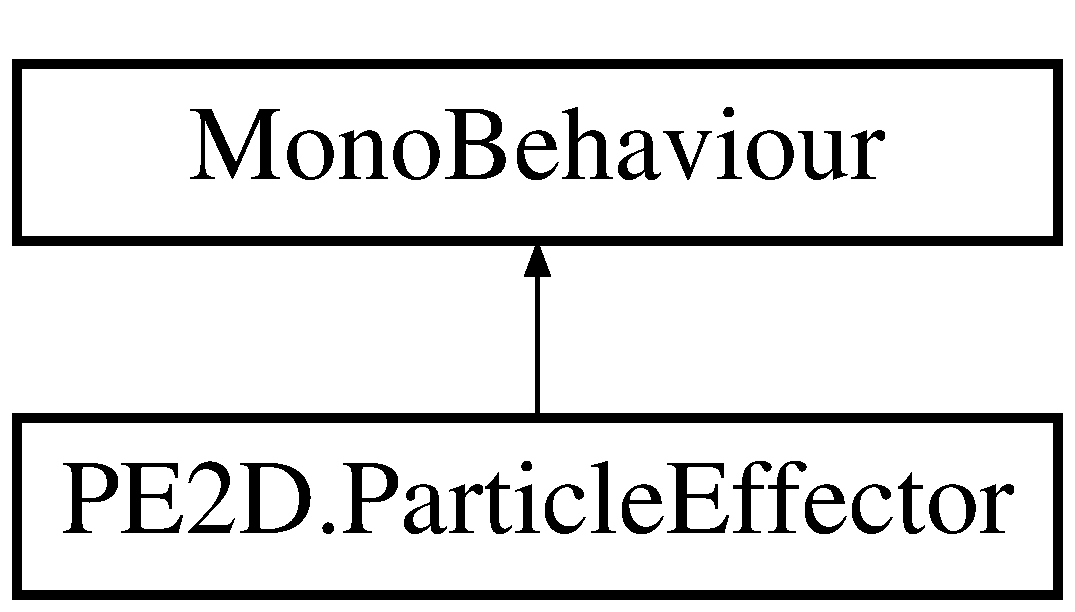
\includegraphics[height=2.000000cm]{class_p_e2_d_1_1_particle_effector}
\end{center}
\end{figure}
\subsection*{Public Attributes}
\begin{DoxyCompactItemize}
\item 
\hypertarget{class_p_e2_d_1_1_particle_effector_a2fa87e8c0ac248afe34841448bc2e265}{}\hyperlink{namespace_p_e2_d_a476bb8917ed61c9fea94f42486983a11}{Effector\+Type} {\bfseries effector\+Type}\label{class_p_e2_d_1_1_particle_effector_a2fa87e8c0ac248afe34841448bc2e265}

\item 
\hypertarget{class_p_e2_d_1_1_particle_effector_ac6db8f7e8b6e51bbef84f6ded5c811ea}{}float {\bfseries distance}\label{class_p_e2_d_1_1_particle_effector_ac6db8f7e8b6e51bbef84f6ded5c811ea}

\item 
\hypertarget{class_p_e2_d_1_1_particle_effector_a6f68fbe9b32953cef5517094684a673b}{}float {\bfseries rotate\+Distance}\label{class_p_e2_d_1_1_particle_effector_a6f68fbe9b32953cef5517094684a673b}

\item 
\hypertarget{class_p_e2_d_1_1_particle_effector_a0395c3e2e9c6e452338c800a17bd55d5}{}float {\bfseries force}\label{class_p_e2_d_1_1_particle_effector_a0395c3e2e9c6e452338c800a17bd55d5}

\end{DoxyCompactItemize}


\subsection{Detailed Description}
Add to a gameobject to effect a particles movement. 



The documentation for this class was generated from the following file\+:\begin{DoxyCompactItemize}
\item 
/\+Users/robert/\+Dropbox/\+Work/\+Unity/\+Particle Effects 2\+D/\+Assets/\+P\+E2\+D/\+Scripts/\+Particles/Particle\+Effector.\+cs\end{DoxyCompactItemize}

\hypertarget{class_p_e2_d_1_1_particle_emitter_in_object_direction}{}\section{P\+E2\+D.\+Particle\+Emitter\+In\+Object\+Direction Class Reference}
\label{class_p_e2_d_1_1_particle_emitter_in_object_direction}\index{P\+E2\+D.\+Particle\+Emitter\+In\+Object\+Direction@{P\+E2\+D.\+Particle\+Emitter\+In\+Object\+Direction}}


Emits particles based on objects rotation.  


Inheritance diagram for P\+E2\+D.\+Particle\+Emitter\+In\+Object\+Direction\+:\begin{figure}[H]
\begin{center}
\leavevmode
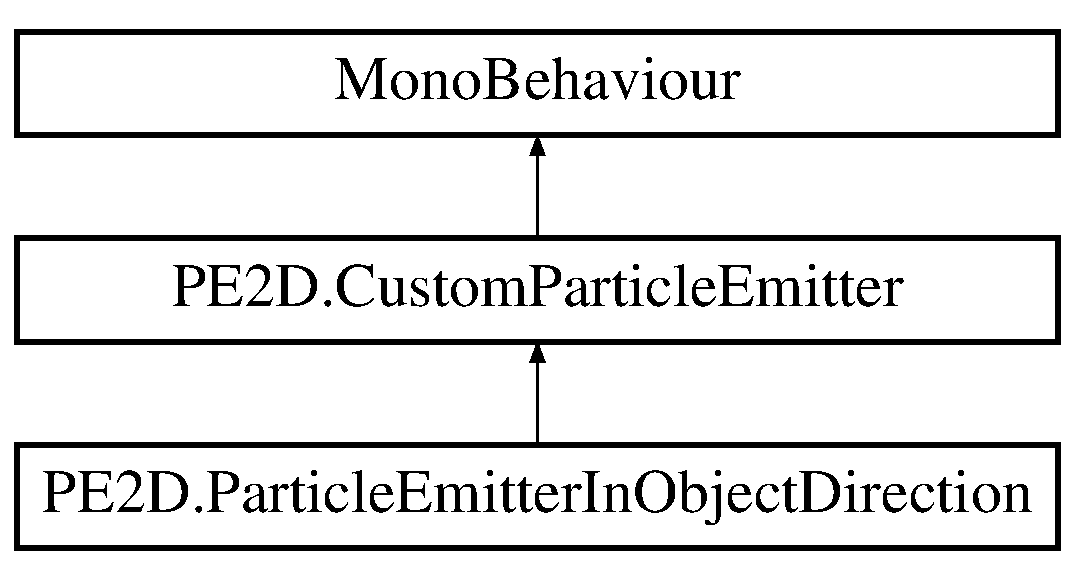
\includegraphics[height=3.000000cm]{class_p_e2_d_1_1_particle_emitter_in_object_direction}
\end{center}
\end{figure}
\subsection*{Protected Member Functions}
\begin{DoxyCompactItemize}
\item 
\hypertarget{class_p_e2_d_1_1_particle_emitter_in_object_direction_a9f5e6461f1998fbda78e1da8c13176ef}{}override void {\bfseries Release\+Particle} ()\label{class_p_e2_d_1_1_particle_emitter_in_object_direction_a9f5e6461f1998fbda78e1da8c13176ef}

\end{DoxyCompactItemize}
\subsection*{Additional Inherited Members}


\subsection{Detailed Description}
Emits particles based on objects rotation. 



The documentation for this class was generated from the following file\+:\begin{DoxyCompactItemize}
\item 
/\+Users/robert/\+Dropbox/\+Work/\+Unity/\+Particle Effects 2\+D/\+Assets/\+P\+E2\+D/\+Scripts/\+Particles/\+Emitters/Particle\+Emitter\+In\+Object\+Direction.\+cs\end{DoxyCompactItemize}

\hypertarget{class_p_e2_d_1_1_particle_emitter_in_random_direction}{}\section{P\+E2\+D.\+Particle\+Emitter\+In\+Random\+Direction Class Reference}
\label{class_p_e2_d_1_1_particle_emitter_in_random_direction}\index{P\+E2\+D.\+Particle\+Emitter\+In\+Random\+Direction@{P\+E2\+D.\+Particle\+Emitter\+In\+Random\+Direction}}


Emits particles from objects position in a random direction.  


Inheritance diagram for P\+E2\+D.\+Particle\+Emitter\+In\+Random\+Direction\+:\begin{figure}[H]
\begin{center}
\leavevmode
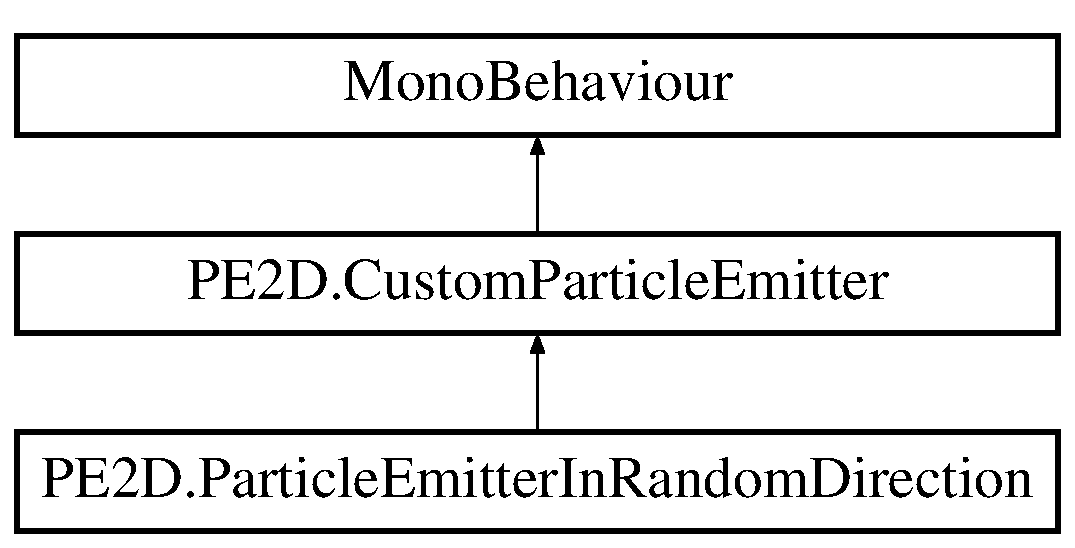
\includegraphics[height=3.000000cm]{class_p_e2_d_1_1_particle_emitter_in_random_direction}
\end{center}
\end{figure}
\subsection*{Protected Member Functions}
\begin{DoxyCompactItemize}
\item 
\hypertarget{class_p_e2_d_1_1_particle_emitter_in_random_direction_a1a3361f42094f2cf1f47ea4bfac4e4df}{}override void {\bfseries Release\+Particle} ()\label{class_p_e2_d_1_1_particle_emitter_in_random_direction_a1a3361f42094f2cf1f47ea4bfac4e4df}

\end{DoxyCompactItemize}
\subsection*{Additional Inherited Members}


\subsection{Detailed Description}
Emits particles from objects position in a random direction. 



The documentation for this class was generated from the following file\+:\begin{DoxyCompactItemize}
\item 
/\+Users/robert/\+Dropbox/\+Work/\+Unity/\+Particle Effects 2\+D/\+Assets/\+P\+E2\+D/\+Scripts/\+Particles/\+Emitters/Particle\+Emitter\+In\+Random\+Direction.\+cs\end{DoxyCompactItemize}

\hypertarget{class_p_e2_d_1_1_particle_factory}{}\section{P\+E2\+D.\+Particle\+Factory Class Reference}
\label{class_p_e2_d_1_1_particle_factory}\index{P\+E2\+D.\+Particle\+Factory@{P\+E2\+D.\+Particle\+Factory}}


Creates and maintain an object pool of particles.  


Inheritance diagram for P\+E2\+D.\+Particle\+Factory\+:\begin{figure}[H]
\begin{center}
\leavevmode
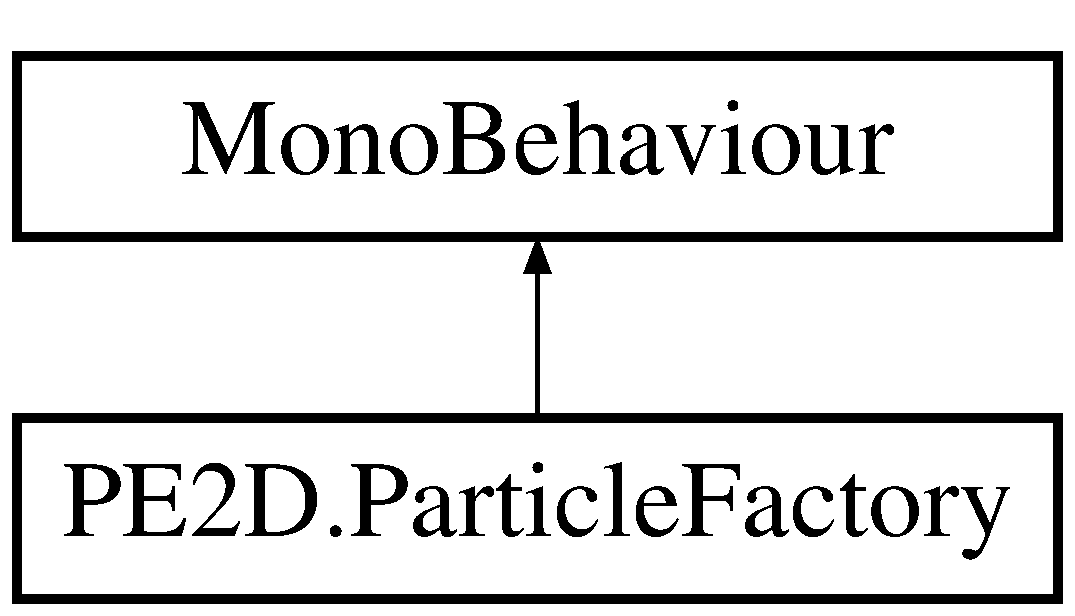
\includegraphics[height=2.000000cm]{class_p_e2_d_1_1_particle_factory}
\end{center}
\end{figure}
\subsection*{Public Member Functions}
\begin{DoxyCompactItemize}
\item 
void \hyperlink{class_p_e2_d_1_1_particle_factory_a5d0fd6f0ecf11f2545ff889e02eaf09a}{Create\+Particle} (Vector2 position, Color colour, float duration, Vector2 initial\+Scale, \hyperlink{struct_p_e2_d_1_1_particle_builder}{Particle\+Builder} state)
\begin{DoxyCompactList}\small\item\em Creates a particle at position with the specified state. \end{DoxyCompactList}\item 
void \hyperlink{class_p_e2_d_1_1_particle_factory_a6d8498b66145f0035b9346118aad9150}{Remove\+All\+Active\+Particles} ()
\begin{DoxyCompactList}\small\item\em Sets all enabled particles to be removed in the next time step. \end{DoxyCompactList}\end{DoxyCompactItemize}
\subsection*{Public Attributes}
\begin{DoxyCompactItemize}
\item 
Game\+Object \hyperlink{class_p_e2_d_1_1_particle_factory_a7431706eb3ca0363ebfa1936384fa8ca}{particle\+Prefab}
\begin{DoxyCompactList}\small\item\em Particle prefab. \end{DoxyCompactList}\item 
int \hyperlink{class_p_e2_d_1_1_particle_factory_a7a8905551b65537a74461cddeaaac5d3}{max\+Particle\+Count}
\begin{DoxyCompactList}\small\item\em The max particle count. This number of particles is created at runtime and placed in a finite pool. \end{DoxyCompactList}\end{DoxyCompactItemize}
\subsection*{Properties}
\begin{DoxyCompactItemize}
\item 
static \hyperlink{class_p_e2_d_1_1_particle_factory}{Particle\+Factory} \hyperlink{class_p_e2_d_1_1_particle_factory_a5ee02796828431320c6f8a70a8456feb}{instance}\hspace{0.3cm}{\ttfamily  \mbox{[}get\mbox{]}}
\begin{DoxyCompactList}\small\item\em Gets the instance of this class. Can be called from any script. Only one instance of a particle factory can exist in one scene. \end{DoxyCompactList}\end{DoxyCompactItemize}


\subsection{Detailed Description}
Creates and maintain an object pool of particles. 



\subsection{Member Function Documentation}
\hypertarget{class_p_e2_d_1_1_particle_factory_a5d0fd6f0ecf11f2545ff889e02eaf09a}{}\index{P\+E2\+D\+::\+Particle\+Factory@{P\+E2\+D\+::\+Particle\+Factory}!Create\+Particle@{Create\+Particle}}
\index{Create\+Particle@{Create\+Particle}!P\+E2\+D\+::\+Particle\+Factory@{P\+E2\+D\+::\+Particle\+Factory}}
\subsubsection[{Create\+Particle(\+Vector2 position, Color colour, float duration, Vector2 initial\+Scale, Particle\+Builder state)}]{\setlength{\rightskip}{0pt plus 5cm}void P\+E2\+D.\+Particle\+Factory.\+Create\+Particle (
\begin{DoxyParamCaption}
\item[{Vector2}]{position, }
\item[{Color}]{colour, }
\item[{float}]{duration, }
\item[{Vector2}]{initial\+Scale, }
\item[{{\bf Particle\+Builder}}]{state}
\end{DoxyParamCaption}
)}\label{class_p_e2_d_1_1_particle_factory_a5d0fd6f0ecf11f2545ff889e02eaf09a}


Creates a particle at position with the specified state. 


\begin{DoxyParams}{Parameters}
{\em position} & Initial position of particle.\\
\hline
{\em tint} & The initial colour of particle.\\
\hline
{\em duration} & The maximum duration of particle.\\
\hline
{\em scale} & Initial scale of particle.\\
\hline
{\em state} & T\+He particle state.\\
\hline
\end{DoxyParams}
\hypertarget{class_p_e2_d_1_1_particle_factory_a6d8498b66145f0035b9346118aad9150}{}\index{P\+E2\+D\+::\+Particle\+Factory@{P\+E2\+D\+::\+Particle\+Factory}!Remove\+All\+Active\+Particles@{Remove\+All\+Active\+Particles}}
\index{Remove\+All\+Active\+Particles@{Remove\+All\+Active\+Particles}!P\+E2\+D\+::\+Particle\+Factory@{P\+E2\+D\+::\+Particle\+Factory}}
\subsubsection[{Remove\+All\+Active\+Particles()}]{\setlength{\rightskip}{0pt plus 5cm}void P\+E2\+D.\+Particle\+Factory.\+Remove\+All\+Active\+Particles (
\begin{DoxyParamCaption}
{}
\end{DoxyParamCaption}
)}\label{class_p_e2_d_1_1_particle_factory_a6d8498b66145f0035b9346118aad9150}


Sets all enabled particles to be removed in the next time step. 



\subsection{Member Data Documentation}
\hypertarget{class_p_e2_d_1_1_particle_factory_a7a8905551b65537a74461cddeaaac5d3}{}\index{P\+E2\+D\+::\+Particle\+Factory@{P\+E2\+D\+::\+Particle\+Factory}!max\+Particle\+Count@{max\+Particle\+Count}}
\index{max\+Particle\+Count@{max\+Particle\+Count}!P\+E2\+D\+::\+Particle\+Factory@{P\+E2\+D\+::\+Particle\+Factory}}
\subsubsection[{max\+Particle\+Count}]{\setlength{\rightskip}{0pt plus 5cm}int P\+E2\+D.\+Particle\+Factory.\+max\+Particle\+Count}\label{class_p_e2_d_1_1_particle_factory_a7a8905551b65537a74461cddeaaac5d3}


The max particle count. This number of particles is created at runtime and placed in a finite pool. 

\hypertarget{class_p_e2_d_1_1_particle_factory_a7431706eb3ca0363ebfa1936384fa8ca}{}\index{P\+E2\+D\+::\+Particle\+Factory@{P\+E2\+D\+::\+Particle\+Factory}!particle\+Prefab@{particle\+Prefab}}
\index{particle\+Prefab@{particle\+Prefab}!P\+E2\+D\+::\+Particle\+Factory@{P\+E2\+D\+::\+Particle\+Factory}}
\subsubsection[{particle\+Prefab}]{\setlength{\rightskip}{0pt plus 5cm}Game\+Object P\+E2\+D.\+Particle\+Factory.\+particle\+Prefab}\label{class_p_e2_d_1_1_particle_factory_a7431706eb3ca0363ebfa1936384fa8ca}


Particle prefab. 



\subsection{Property Documentation}
\hypertarget{class_p_e2_d_1_1_particle_factory_a5ee02796828431320c6f8a70a8456feb}{}\index{P\+E2\+D\+::\+Particle\+Factory@{P\+E2\+D\+::\+Particle\+Factory}!instance@{instance}}
\index{instance@{instance}!P\+E2\+D\+::\+Particle\+Factory@{P\+E2\+D\+::\+Particle\+Factory}}
\subsubsection[{instance}]{\setlength{\rightskip}{0pt plus 5cm}{\bf Particle\+Factory} P\+E2\+D.\+Particle\+Factory.\+instance\hspace{0.3cm}{\ttfamily [static]}, {\ttfamily [get]}}\label{class_p_e2_d_1_1_particle_factory_a5ee02796828431320c6f8a70a8456feb}


Gets the instance of this class. Can be called from any script. Only one instance of a particle factory can exist in one scene. 

The instance.

The documentation for this class was generated from the following file\+:\begin{DoxyCompactItemize}
\item 
/\+Users/robert/\+Dropbox/\+Work/\+Unity/\+Particle Effects 2\+D/\+Assets/\+P\+E2\+D/\+Scripts/\+Particles/Particle\+Factory.\+cs\end{DoxyCompactItemize}

\hypertarget{class_p_e2_d_1_1_particle_renderer}{}\section{P\+E2\+D.\+Particle\+Renderer Class Reference}
\label{class_p_e2_d_1_1_particle_renderer}\index{P\+E2\+D.\+Particle\+Renderer@{P\+E2\+D.\+Particle\+Renderer}}


Simple renderer script for particles that disables the sprite renderer on enable and re-\/enables the srpite renderer after a time specified by Particle\+Renderer\+::\+R\+E\+N\+D\+E\+R\+E\+R\+\_\+\+D\+E\+L\+A\+Y. Attach to the particle prefab to prevent occasional graphic glitches.  


Inheritance diagram for P\+E2\+D.\+Particle\+Renderer\+:\begin{figure}[H]
\begin{center}
\leavevmode
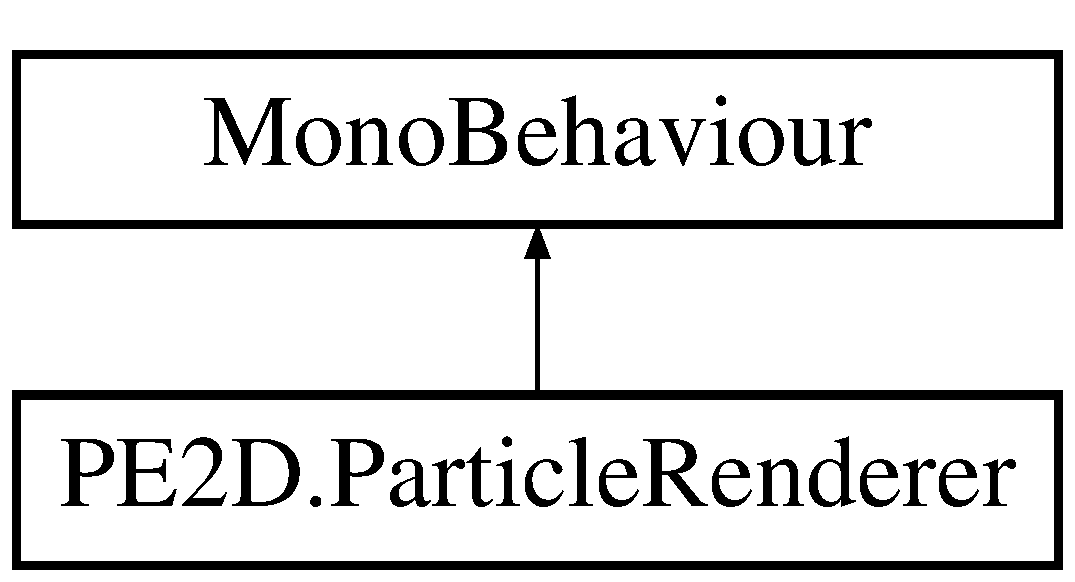
\includegraphics[height=2.000000cm]{class_p_e2_d_1_1_particle_renderer}
\end{center}
\end{figure}


\subsection{Detailed Description}
Simple renderer script for particles that disables the sprite renderer on enable and re-\/enables the srpite renderer after a time specified by Particle\+Renderer\+::\+R\+E\+N\+D\+E\+R\+E\+R\+\_\+\+D\+E\+L\+A\+Y. Attach to the particle prefab to prevent occasional graphic glitches. 



The documentation for this class was generated from the following file\+:\begin{DoxyCompactItemize}
\item 
/\+Users/robert/\+Dropbox/\+Work/\+Unity/\+Particle Effects 2\+D/\+Assets/\+P\+E2\+D/\+Scripts/\+Particles/Particle\+Renderer.\+cs\end{DoxyCompactItemize}

\hypertarget{class_p_e2_d_1_1_pulsate}{}\section{P\+E2\+D.\+Pulsate Class Reference}
\label{class_p_e2_d_1_1_pulsate}\index{P\+E2\+D.\+Pulsate@{P\+E2\+D.\+Pulsate}}


Simple script used to pulse an objects size. Used in the demo scene for the effectors.  


Inheritance diagram for P\+E2\+D.\+Pulsate\+:\begin{figure}[H]
\begin{center}
\leavevmode
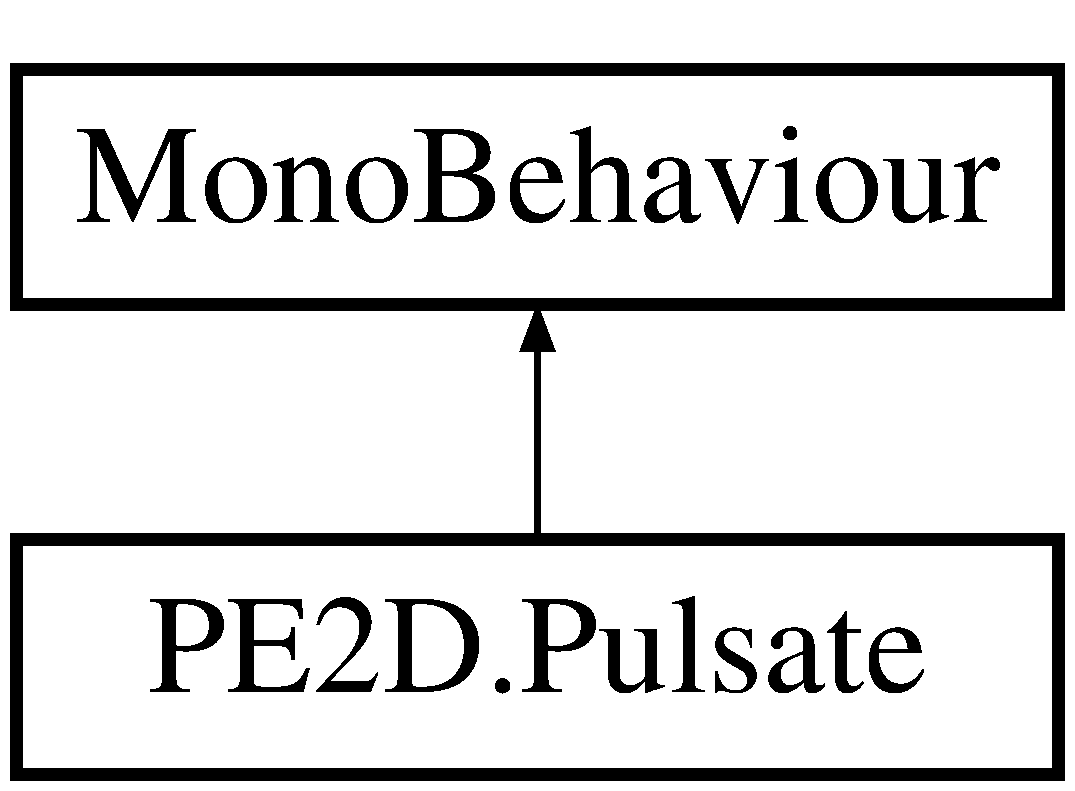
\includegraphics[height=2.000000cm]{class_p_e2_d_1_1_pulsate}
\end{center}
\end{figure}


\subsection{Detailed Description}
Simple script used to pulse an objects size. Used in the demo scene for the effectors. 



The documentation for this class was generated from the following file\+:\begin{DoxyCompactItemize}
\item 
/\+Users/robert/\+Dropbox/\+Work/\+Unity/\+Particle Effects 2\+D/\+Assets/\+P\+E2\+D/\+Scripts/Pulsate.\+cs\end{DoxyCompactItemize}

%--- End generated contents ---

% Index
\backmatter
\newpage
\phantomsection
\clearemptydoublepage
\addcontentsline{toc}{chapter}{Index}
\printindex

\end{document}
